\chapter{博弈论与多方决策}
\label{chap:game-theory-and-multi-agent-decision}

第~\ref{chap:decision-theory-and-dynamic-risk}章把环境规律看作给定条件，
第~\ref{chap:control-theory}章则让单个控制器通过反馈改变状态。多方决策进一步改变了
“其他行动规则固定”这一前提。若另一方也会观察、推断和
调整，当前行动的后果就取决于双方策略，而不能只对一个固定环境分布取期望。此时，
“哪个行动最好”必须改写为“面对其他参与者的选择，什么策略能够抵抗偏离或形成稳定响应”。
本章沿用一个三张牌的教学博弈。牌面只有高牌、中牌和低牌，实际使用其中一张隐藏牌来
决定是否质询、是否应对。这个小牌面会先被压缩成收益矩阵，用于求零和博弈值；随后还原
成历史树，说明私人信息为何不能当作普通状态。重复对局时，局部决策会产生遗憾，完全回忆
把这些局部遗憾连接到整局偏离。若参与者转为合作，同一个任务又会提出怎样按各方信息
分配共同收益的问题。
这几类答案不可互换。极小极大值控制最坏对手下的保证，Nash均衡排除单方有利偏离，
相关均衡还要说明看到建议后允许怎样改动；低遗憾是多轮比较结论，不自动说明末次策略
收敛；Shapley值分配预先定义的联盟价值，却不负责证明参与者会自愿采用该分配。本章
依次从收益结构、响应稳定性、信息结构、学习过程和合作分配五个方面建立这些边界。

\section{在零和对抗中求最坏对手下的保证}
\label{sec:game-matrix-zero-sum-duality}
\subsection{联合行动、混合策略与最佳响应}

\begin{definition}[有限矩阵博弈]
\label{def:game-finite-matrix-game}
有限双人\term{矩阵博弈}（matrix game）由两组非空有限行动
\(A_1=\{1,\ldots,m\}\)、\(A_2=\{1,\ldots,n\}\)和两张收益矩阵
\(\bm{U}_1,\bm{U}_2\in\mathbb{R}^{m\times n}\)给出。第1位参与者选择行，第2位
参与者选择列，落在\((i,j)\)时，两人的收益分别为
\(\bigl((\bm{U}_1)_{i,j},(\bm{U}_2)_{i,j}\bigr)\)。若存在矩阵\(\bm{M}\)使
\(\bm{U}_1=\bm{M}\)、\(\bm{U}_2=-\bm{M}\)，双方收益之和恒为零，就得到
\term{零和博弈}（zero-sum game）。
\end{definition}
一个人增加的收益正好是另一个人的损失，因此
零和情形只需记录第1位参与者的收益矩阵\(\bm{M}\)；一般和情形则不能省略第二张矩阵。

固定行动容易被对方针对，随机选择则把可预测的单一行动改成一个概率分布。
\begin{definition}[纯策略与混合策略]
\label{def:game-pure-mixed-strategy}
直接选择某一行或某一列称为\term{纯策略}（pure strategy）。在行动上选择概率分布
称为混合策略（mixed strategy）。记
\[
  \Delta_m
  =
  \left\{
    \bm{x}\in\mathbb{R}^m:
    \bm{x}\geq\bm{0},\
    \bm{1}^{\top}\bm{x}=1
  \right\}
\]
为\(m\)个行动上的概率单纯形。双方以各自的混合策略独立抽取行动。
\end{definition}
该单纯形嵌入\(\mathbb{R}^m\)，几何维数为\(m-1\)。在零和情形，第1位参与者采用
\(\bm{x}\in\Delta_m\)，第2位参与者采用
\(\bm{y}\in\Delta_n\)时，期望收益为
\begin{equation}
  u(\bm{x},\bm{y})
  =
  \bm{x}^{\top}\bm{M}\bm{y}.
  \label{eq:game-matrix-expected-payoff}
\end{equation}
混合策略不是在一局内把多个行动平均执行，而是在行动前用随机装置抽取一个纯行动。

\begin{definition}[最佳响应]
\label{def:game-best-response}
给定对手策略后，使自身期望收益最大的策略称为\term{最佳响应}（best response）。
在零和情形，第1位参与者面对\(\bm{y}\)的最佳响应集合为
\[
  \operatorname{BR}_1(\bm{y})
  =
  \argmax_{\bm{x}\in\Delta_m}
  \bm{x}^{\top}\bm{M}\bm{y}.
\]
\end{definition}
一般和矩阵博弈中，将上述目标中的$\bm M$换成自己的收益矩阵$\bm U_1$；
第2位参与者则最大化$\bm x^\top\bm U_2\bm y$，不能继续把对方收益简单取负。
线性目标总能在某个纯行动达到最大值，但把全部概率放在一个最佳纯行动上未必是唯一
选择；若多行并列，它们的任意混合仍是最佳响应。

\subsection{匹配硬币与混合策略}

考虑双方同时选择正面\(H\)或反面\(T\)。两面相同时参与者1得到\(1\)，不同时得到
\(-1\)，参与者2得到相反收益。参与者1的收益矩阵为
\[
  \bm{M}_{\mathrm{mp}}
  =
  \begin{pmatrix}
    1 & -1\\
    -1 & 1
  \end{pmatrix}.
\]
任意纯策略组合都不是稳定响应：若两面相同，参与者2改换一面便能改善；若两面不同，
参与者1改换一面便能改善。若逐轮对上一轮行动作纯最佳响应，行动还会在四个组合之间
循环，这说明“每轮都回应当前对手”不等于联合策略会收敛。

令参与者1选择\(H\)的概率为\(p\)，参与者2选择\(H\)的概率为\(q\)。参与者1选
\(H\)与\(T\)的期望收益分别为\(2q-1\)与\(1-2q\)。只有\(q=1/2\)能使两行
收益相同，避免参与者1利用某一面；对称地，只有\(p=1/2\)能使参与者2无法利用。
所以双方均匀随机化时收益为
\[
  (1/2,1/2)\bm{M}_{\mathrm{mp}}(1/2,1/2)^{\top}=0.
\]
这个二乘二例子展示了混合策略的核心作用：随机化不是让某个纯行动变好，而是消除对手
针对固定行动获得的优势。

图~\ref{fig:game-matching-best-responses}把双方最佳响应放到同一概率平面中。
给定纵坐标$q$，蓝线列出行方允许采用的最佳$p$；给定横坐标$p$，红线列出列方的
最佳$q$。各自单看一条响应仍不能选出联合结果；两条集合同时相交，才表示双方都在
回应对方。中心的整段响应保留了并列最优，因此这个均衡不要求“每个人有唯一最佳行动”。

\begin{figure}[htbp]
  \centering
  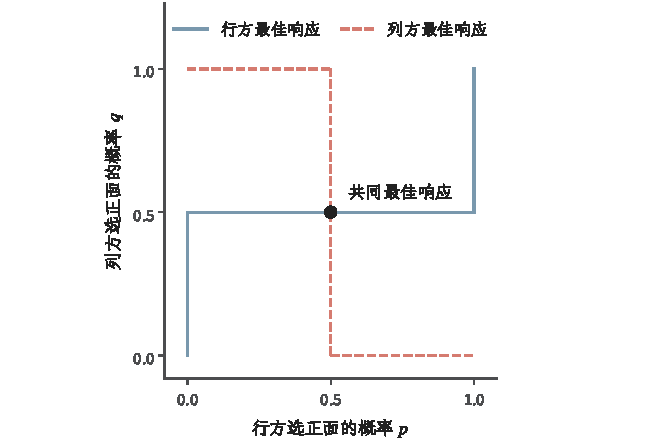
\includegraphics[width=\linewidth]{figures/math-preparation/dynamics/matching-best-responses.pdf}
  \caption{匹配硬币中的最佳响应对应。横轴$p$是行方选$H$的概率，纵轴$q$是列方选
  $H$的概率；蓝色实线表示行方最大化收益的最佳响应，红色虚线表示列方最小化行方收益
  的最佳响应。蓝线在$q=1/2$包含全部$p$，红线在$p=1/2$包含全部$q$，唯一交点
  为$(1/2,1/2)$。线段是最佳响应集合，不是随时间运行的学习轨迹。}
  \label{fig:game-matching-best-responses}
\end{figure}

\subsection{三张牌质询博弈}

考虑高牌\(H\)、中牌\(M\)和低牌\(L\)。庄家从\(H\)与\(L\)中等概率发给参与者1
一张隐藏牌，\(M\)留作公共比较基准。参与者1看到自己的牌后选择质询\(B\)或放弃
\(P\)。放弃时收益为\(0\)。质询后，参与者2只知道发生了质询，不知道隐藏牌，并选择
应对\(C\)或退让\(F\)。退让时参与者1得到\(1\)；应对时，高牌使参与者1得到\(2\)，
低牌使其得到\(-2\)。参与者2得到相反收益。

在把信息时序展开以前，可以先把一项纯策略写成“拿到高牌时做什么，拿到低牌时做什么”。
按\((P,P),(B,P),(P,B),(B,B)\)排列参与者1的四个完整计划，按\(F,C\)排列参与者2
的行动，参与者1的事前期望收益矩阵为
\begin{equation}
  \bm{M}
  =
  \begin{pmatrix}
    0 & 0\\
    1/2 & 1\\
    1/2 & -1\\
    1 & 0
  \end{pmatrix}.
  \label{eq:game-card-normal-form}
\end{equation}
例如，计划\((B,P)\)只在拿到高牌时质询。对方退让时，收益以一半概率为\(1\)、一半
概率为\(0\)，故矩阵元素为\(1/2\)；对方应对时，相应期望为\(1\)。

这个矩阵没有纯策略鞍点。每一行的最小收益依次为
\(0,1/2,-1,0\)，故第1位参与者先公开选行时至多保证\(1/2\)；每一列的最大收益
分别为\(1,1\)，故第2位参与者先公开选列时至多把收益压到\(1\)。两种次序得到不同
数值，说明任何固定纯行动都会留下可利用的响应。

\subsection{保证值与极小极大值}

第1位参与者在不知道对方将怎样响应时，希望最大化自己能够保证的最小收益：
\[
  \underline v
  =
  \max_{\bm{x}\in\Delta_m}
  \min_{\bm{y}\in\Delta_n}
  \bm{x}^{\top}\bm{M}\bm{y}.
\]
对固定\(\bm{x}\)，第2位参与者的目标关于\(\bm{y}\)线性，所以最小值在某个纯列
达到。因此
\[
  \min_{\bm{y}\in\Delta_n}
  \bm{x}^{\top}\bm{M}\bm{y}
  =
  \min_j(\bm{M}^{\top}\bm{x})_j.
\]
类似地，第2位参与者希望把第1位参与者的最大可得收益压低到
\[
  \overline v
  =
  \min_{\bm{y}\in\Delta_n}
  \max_{\bm{x}\in\Delta_m}
  \bm{x}^{\top}\bm{M}\bm{y}
  =
  \min_{\bm{y}\in\Delta_n}\max_i(\bm{M}\bm{y})_i.
\]

对任意\(\bm{x},\bm{y}\)，都有
\[
  \min_{\widetilde{\bm{y}}}
  u(\bm{x},\widetilde{\bm{y}})
  \leq
  u(\bm{x},\bm{y})
  \leq
  \max_{\widetilde{\bm{x}}}
  u(\widetilde{\bm{x}},\bm{y}).
\]
分别对左侧取最大、右侧取最小，得到
\(\underline v\leq\overline v\)。这只是弱极小极大关系。要证明有限零和博弈中
两者相等，还需要说明双方约束恰好构成一对线性规划。

\begin{theorem}[有限零和博弈的极小极大定理]
\label{thm:game-finite-minimax}
对任意有限收益矩阵\(\bm{M}\)，有
\begin{equation}
  \max_{\bm{x}\in\Delta_m}
  \min_{\bm{y}\in\Delta_n}
  \bm{x}^{\top}\bm{M}\bm{y}
  =
  \min_{\bm{y}\in\Delta_n}
  \max_{\bm{x}\in\Delta_m}
  \bm{x}^{\top}\bm{M}\bm{y}.
  \label{eq:game-minimax-equality}
\end{equation}
共同数值称为博弈值\(v^\star\)。等式两侧的最优解分别称为双方的极小极大策略。
\end{theorem}

\begin{proof}
引入第1位参与者要保证的收益下界\(v\)。条件
\((\bm{M}^{\top}\bm{x})_j\geq v\)对每一列成立，恰好表示任何纯列都不能把收益压到
\(v\)以下。第1位参与者的问题因此是
\begin{equation}
  \begin{aligned}
    \max_{\bm{x},v}\quad&v\\
    \text{s.t.}\quad&
      \bm{M}^{\top}\bm{x}\geq v\bm{1},\\
    &\bm{1}^{\top}\bm{x}=1,\qquad
      \bm{x}\geq\bm{0}.
  \end{aligned}
  \label{eq:game-row-player-lp}
\end{equation}
它的最优值正是\(\underline v\)。为第一组不等式引入非负乘子
\(\bm{y}\geq\bm{0}\)，为概率归一化引入自由乘子\(w\)。
把最大化问题写成上界形式后，其拉格朗日函数可整理为
\[
  \mathcal{L}(\bm{x},v;\bm{y},w)
  =
  v+\bm{y}^{\top}
  (\bm{M}^{\top}\bm{x}-v\bm{1})
  +w(1-\bm{1}^{\top}\bm{x}).
\]
若对自由变量\(v\)取上确界仍为有限值，必须有
\(\bm{1}^{\top}\bm{y}=1\)。若对\(\bm{x}\geq\bm{0}\)取上确界仍为有限值，
还必须有
\[
  \bm{M}\bm{y}\leq w\bm{1}.
\]
满足这些条件时，上确界等于\(w\)。于是对偶问题为
\begin{equation}
  \begin{aligned}
    \min_{\bm{y},w}\quad&w\\
    \text{s.t.}\quad&
      \bm{M}\bm{y}\leq w\bm{1},\\
    &\bm{1}^{\top}\bm{y}=1,\qquad
      \bm{y}\geq\bm{0}.
  \end{aligned}
  \label{eq:game-column-player-lp}
\end{equation}
它要求每个纯行的收益都不超过\(w\)，所以最优值正是\(\overline v\)。两个单纯形
都非空且紧，目标连续，因此式~\eqref{eq:game-row-player-lp}与
\eqref{eq:game-column-player-lp}都有有限最优解。第
\ref{thm:opt-lp-strong-duality}号定理给出原对偶最优值相等，即
\(\underline v=\overline v=v^\star\)。
\end{proof}

这个证明不只是交换了\(\max\)与\(\min\)。概率归一化把乘子变成对方的混合策略，
逐行动收益约束把对偶可行性变成“没有纯行动能突破当前上界”。强对偶才把两种单方
证书接成同一个博弈值。

若\(\bm{x}^\star\)与\(\bm{y}^\star\)分别是两侧最优策略，则对任意
\(\bm{x}\in\Delta_m\)、\(\bm{y}\in\Delta_n\)，
\begin{equation}
  u(\bm{x},\bm{y}^\star)
  \leq
  u(\bm{x}^\star,\bm{y}^\star)
  \leq
  u(\bm{x}^\star,\bm{y}).
  \label{eq:game-zero-sum-saddle}
\end{equation}
左侧来自\(\bm{y}^\star\)把所有行收益限制在\(v^\star\)以下，右侧来自
\(\bm{x}^\star\)对所有列保证至少\(v^\star\)。这就是混合策略上的鞍点条件。
博弈值由式~\eqref{eq:game-minimax-equality}唯一确定，但达到该值的策略可以不唯一；
把“值唯一”误读成“解唯一”，会遗漏并列最优行动形成的整个最优策略集合。

\subsection{牌面博弈的原对偶最优证书}

对式~\eqref{eq:game-card-normal-form}，令第1位参与者在计划
\((B,P)\)与\((B,B)\)上分别放置概率\(2/3\)与\(1/3\)，其余计划概率为零：
\[
  \bm{x}^\star
  =
  (0,2/3,0,1/3)^{\top}.
\]
面对退让列，期望收益为
\[
  \frac23\cdot\frac12+\frac13\cdot1
  =
  \frac23;
\]
面对应对列，期望收益为
\[
  \frac23\cdot1+\frac13\cdot0
  =
  \frac23.
\]
所以\((\bm{x}^\star,2/3)\)是式~\eqref{eq:game-row-player-lp}的可行解。

再令第2位参与者以概率\(2/3\)退让、以概率\(1/3\)应对：
\[
  \bm{y}^\star=(2/3,1/3)^{\top}.
\]
四个纯计划对它的收益依次为
\[
  0,\qquad
  \frac12\cdot\frac23+1\cdot\frac13=\frac23,\qquad
  \frac12\cdot\frac23-1\cdot\frac13=0,\qquad
  \frac23.
\]
没有一行超过\(2/3\)，所以\((\bm{y}^\star,2/3)\)是
式~\eqref{eq:game-column-player-lp}的可行解。弱对偶已经足以说明两者同时最优，
博弈值为\(v^\star=2/3\)。

从牌面条件看，这个混合计划等价于：拿到高牌总是质询，拿到低牌以概率\(1/3\)质询；
参与者2面对质询时以概率\(1/3\)应对。高牌的强行动掩护了低牌的偶尔质询，低牌的
存在又使应对者不能总是退让。这个解释依赖参与者2看不到牌面；第
~\ref{sec:game-extensive-information}节会把该信息限制写进历史树。

极小极大结论依赖零和结构。若退让、应对或交易产生了双方并不相反的成本，就不能再用
一个标量博弈值同时概括双方目标。此时仍可讨论最佳响应，但稳定性必须改用一般和均衡。
对于无限或连续行动集，有限维线性规划证明也不再直接适用；交换极大与极小通常还需要
非空紧凸策略集、收益连续以及相应的凸凹结构。

\section{排除单方偏离并判断均衡是否存在}
\label{sec:game-best-response-equilibrium}

零和对偶把一方所得与另一方所失连在一起，给出双方共享的博弈值。
一般和收益没有这项共同标尺，因而改用“任何一方单独改变策略都不获利”描述稳定响应。
最佳响应对应与不动点工具用于证明这种策略组合存在；相关建议进一步改变允许偏离时掌握的信息。

\subsection{一般和收益与Nash均衡}

\begin{definition}[有限战略式博弈]
\label{def:game-finite-strategic-game}
有限\(n\)人\term{战略式博弈}（strategic-form game）由参与者集合
\(N=\{1,\ldots,n\}\)、每人的有限行动集\(A_i\)和收益函数
\[
  u_i:A_1\times\cdots\times A_n\to\mathbb{R}
\]
组成，各$A_i$均非空。
\end{definition}
一般和博弈允许\(u_i\)与\(u_j\)同时增加或同时减少，因此不存在一个天然的
“共同博弈值”。记混合策略为
\(\bm{\sigma}_i\in\Delta(A_i)\)，联合策略为
\(\bm{\sigma}=(\bm{\sigma}_1,\ldots,\bm{\sigma}_n)\)，去掉第\(i\)项后的组合为
\(\bm{\sigma}_{-i}\)。各参与者按照自己的混合策略独立抽取行动，因此联合行动
\(\bm{a}=(a_1,\ldots,a_n)\)的概率是\(\prod_{j=1}^n\sigma_j(a_j)\)。纯行动收益
由此延拓为期望收益
\begin{equation}
  u_i(\bm{\sigma})
  =
  \sum_{\bm{a}\in A_1\times\cdots\times A_n}
  \left(
    \prod_{j=1}^{n}\sigma_j(a_j)
  \right)
  u_i(\bm{a}).
  \label{eq:game-mixed-payoff-extension}
\end{equation}
后文沿用\(u_i\)表示这一延拓。这里的独立抽样产生乘积分布；相关均衡则允许一般的
联合行动分布。

给定其他参与者的策略，参与者\(i\)的最佳响应对应为
\[
  \operatorname{BR}_i(\bm{\sigma}_{-i})
  =
  \argmax_{\widetilde{\bm{\sigma}}_i\in\Delta(A_i)}
  u_i(\widetilde{\bm{\sigma}}_i,\bm{\sigma}_{-i}).
\]
这里使用“对应”而不是“函数”，因为多个行动可能并列最优。

\begin{definition}[Nash均衡]
\label{def:game-nash-equilibrium}
联合混合策略\(\bm{\sigma}^\star\)是一个
\term{Nash均衡}（Nash equilibrium），若对每个参与者\(i\)和任意替代策略
\(\widetilde{\bm{\sigma}}_i\)，都有
\begin{equation}
  u_i(\bm{\sigma}_i^\star,\bm{\sigma}_{-i}^\star)
  \geq
  u_i(\widetilde{\bm{\sigma}}_i,\bm{\sigma}_{-i}^\star).
  \label{eq:game-nash-no-unilateral-deviation}
\end{equation}
\end{definition}

这一定义只排除单方偏离。它不要求总收益最大，不排除多个参与者联合偏离，也不比较
不同均衡的公平性。在牌桌上，若两位工作人员都可以付出成本核验牌面，一方核验时另一方
可能选择搭便车；“无人能独自改进”并不等于“核验资源使用得最少”或“双方收益最高”。

零和博弈中的一对极小极大策略构成Nash均衡。反过来，任何零和Nash均衡都给出相同
博弈值，因为一方偏离条件分别给出鞍点不等式
\[
  u(\bm{x},\bm{y}^\star)
  \leq
  u(\bm{x}^\star,\bm{y}^\star)
  \leq
  u(\bm{x}^\star,\bm{y}).
\]
一般和博弈没有这个共同数值，不同均衡还可能给每位参与者带来不同收益。

\subsection{连续不动点与集合值最佳响应}

若每个最佳响应都是唯一且连续的，就可以把所有人的响应拼成映射
\[
  B(\bm{\sigma})
  =
  \bigl(
    \operatorname{BR}_1(\bm{\sigma}_{-1}),\ldots,
    \operatorname{BR}_n(\bm{\sigma}_{-n})
  \bigr),
\]
再寻找\(B(\bm{\sigma})=\bm{\sigma}\)。实际博弈常在收益并列处有多个最佳响应，
\(B\)因而不是单值连续函数。强行规定“并列时选编号最小的行动”会造成跳跃，不能直接
应用Brouwer不动点定理。

存在性论证需要两个不同层次的工具。连续单值映射先借助边界计数取得不动点；
最佳响应存在并列时，再用闭图和凸值保留整组选择。下面保留这两条工具的证明，
并在最后逐项核对有限博弈是否满足条件。

\subsubsection{用边界标号建立连续映射的不动点}

\begin{lemma}[Sperner引理]
\label{lem:game-sperner}
把\(d\)维标准单纯形
\[
  \Delta^d
  =
  \left\{
    \bm{x}\in\mathbb{R}^{d+1}:
    \bm{x}\geq\bm{0},\
    \bm{1}^{\top}\bm{x}=1
  \right\}
\]
有限剖分成小单纯形。若每个剖分顶点的标签属于
\(\{0,\ldots,d\}\)，并且位于由顶点集合\(S\)张成的面上的点只能使用\(S\)中的
标签，则同时含有全部\(d+1\)种标签的小单纯形有奇数个，因而至少存在一个。
\end{lemma}

\begin{proof}
对维数\(d\)归纳。\(d=1\)时，线段两个端点分别只能标\(0\)与\(1\)。沿剖分顶点
从左向右读取标签，每次改变对应一条含有两种标签的小线段；由于起点为\(0\)、终点为
\(1\)，改变次数为奇数。

先在\(d=2\)的三角形中看清高维计数。三条边上的剖分顶点只能使用相应两个端点的
标签。例如，顶点\(0\)与\(1\)之间的边只能标\(0\)或\(1\)，一维情形说明这条
边上含两种标签的小边有奇数条。计数所有带标签\(0,1\)的小边与小三角形的邻接：
内部小边被两个小三角形共享，贡献两次；大三角形边界上的小边只邻接一个小三角形，
而带齐\(0,1\)的边界小边只能出现在刚才的\(0,1\)边上。一个全标号小三角形恰有
一条\(0,1\)边，只含标签\(0,1\)且两种标签都出现的小三角形有两条这样的边，其余
小三角形没有。因此邻接总数为奇数迫使全标号小三角形的数量为奇数。一般维证明把
“小边”换成余维一的小面，把“小三角形”换成小单纯形。

假设结论对\(d-1\)维成立。在全部\(d\)维小单纯形中，计数标签集合恰为
\(\{0,\ldots,d-1\}\)的\((d-1)\)维面与小单纯形的邻接次数。内部面邻接两个
小单纯形，贡献偶数；边界面只邻接一个小单纯形。边界上只有大单纯形的
\(x_d=0\)面可能出现全部标签\(0,\ldots,d-1\)，因为其他边界面缺少其中某个允许
标签。该面继承Sperner标号，归纳假设说明其中这类小面有奇数个。因此总邻接次数为
奇数。

一个\(d\)维小单纯形若含有全部标签\(0,\ldots,d\)，恰有一个面带齐
\(0,\ldots,d-1\)，即去掉标签\(d\)顶点所得的面。若它没有标签\(d\)，却带齐
\(0,\ldots,d-1\)，则\(d+1\)个顶点中恰有一个标签重复，去掉任一重复标签顶点都会
得到这样的面，所以贡献两次；其余小单纯形贡献零次。总邻接次数的奇偶性因而等于全标号
小单纯形数目的奇偶性。前者为奇数，后者至少为一。
\end{proof}

\begin{theorem}[Brouwer不动点定理]
\label{thm:game-brouwer}
若\(K\subseteq\mathbb{R}^d\)非空、紧且凸，则每个连续映射
\(f:K\to K\)至少有一个不动点。
\end{theorem}

\begin{proof}
先令\(K=\Delta^d\)。取网格直径趋于零的一列单纯形剖分。若某个剖分顶点
\(\bm{x}\)已经满足\(f(\bm{x})=\bm{x}\)，结论成立；否则因为
\(\sum_jx_j=\sum_jf_j(\bm{x})=1\)，至少存在一个坐标\(j\)满足
\(x_j>f_j(\bm{x})\)，任选这样的\(j\)作为标签。若\(x_j=0\)，这个严格不等式
不可能成立，所以边界标号满足引理~\ref{lem:game-sperner}的条件。

每个剖分因而都有一个全标号小单纯形。对第\(k\)次剖分，记其中标签为\(j\)的顶点为
\(\bm{x}_{k,j}\)。由紧性可取子列，使\(\bm{x}_{k,0}\to\bm{x}^\star\)；小单纯形
直径趋于零，所以每个\(\bm{x}_{k,j}\)都趋于同一个\(\bm{x}^\star\)。标签定义和
连续性给出
\[
  x_j^\star\geq f_j(\bm{x}^\star),
  \qquad j=0,\ldots,d.
\]
两边坐标和都为\(1\)，故所有不等式只能同时取等号，
\(f(\bm{x}^\star)=\bm{x}^\star\)。

对一般的非空紧凸集\(K\)，取一个包含\(K\)的有限维单纯形\(S\)，并记
\(\Pi_K:S\to K\)为到闭凸集\(K\)的欧氏投影。映射
\(g=f\circ\Pi_K:S\to K\subseteq S\)连续，前一部分给出
\(\bm{x}^\star=g(\bm{x}^\star)\)。右侧属于\(K\)，所以
\(\bm{x}^\star\in K\)且\(\Pi_K(\bm{x}^\star)=\bm{x}^\star\)，进而
\(f(\bm{x}^\star)=\bm{x}^\star\)。
\end{proof}

在区间上，这个结论退化为对\(f(x)-x\)使用介值性质；高维中没有统一的“左右端点”，
Sperner引理用边界相容标号和奇偶计数补上了这一步。Brouwer只保证不动点存在，不要求
映射压缩，因此既不保证不动点唯一，也不保证反复应用\(f\)会收敛。

\subsubsection{用闭图保存并列响应}

需要的替代对象保留全部并列响应，不强制挑选其中一个。与单值连续性相应的条件，
要求附近输入的响应不能突然出现远离当前响应集合的新值。
\begin{definition}[集合值映射与上半连续性]
\label{def:game-upper-hemicontinuous-correspondence}
设$K\subseteq\mathbb R^d$非空且紧。\term{集合值映射}（correspondence）
\(F:K\rightrightarrows K\)给每个$x\in K$指定集合$F(x)\subseteq K$；本节要求各值非空。
若对每个$x\in K$及包含$F(x)$的相对开集$O\subseteq K$，都有$x$的相对邻域$U$，
使$F(z)\subseteq O$对所有$z\in U$成立，则称$F$\term{上半连续}（upper hemicontinuous）。
\end{definition}
在当前紧域、紧值的情形，一个便于使用的等价判据是闭图性质：
\[
  x_k\to x,\quad y_k\to y,\quad y_k\in F(x_k)
  \quad\Longrightarrow\quad
  y\in F(x).
\]
闭图判据适用于后面的有限博弈，因为定义域和值域都位于有限维紧集。

例如，对手以概率\(q\)选择左列，而某参与者的两个行动收益分别为\(q\)和\(1-q\)时，
其最佳响应对应为
\[
  \operatorname{BR}(q)
  =
  \begin{cases}
    \{\text{左}\},&q>1/2,\\
    \Delta(\{\text{左},\text{右}\}),&q=1/2,\\
    \{\text{右}\},&q<1/2.
  \end{cases}
\]
在\(q=1/2\)强行挑一个行动会造成单值选择跳跃；保留整段混合策略后，对应的值仍非空、
紧且凸，并且极限不会跳出图。这正是Kakutani定理保留并列响应的方式。

\subsubsection{把集合值响应转成近似连续映射}

闭图控制极限，凸值允许在网格上混合相邻选择。二者配合，才可以把连续映射的存在工具
扩展到集合值响应，而不是对某个不连续的并列选择直接迭代。
下面使用的多值映射不动点结论源于Kakutani定理\scite{math-kakutani1941fixed}
\begin{theorem}[Kakutani不动点定理]
\label{thm:game-kakutani}
设\(K\subseteq\mathbb{R}^d\)非空、紧且凸。若
\(F:K\rightrightarrows K\)上半连续，并且每个\(F(x)\)都非空、紧且凸，
则存在\(x^\star\in K\)满足\(x^\star\in F(x^\star)\)。
\end{theorem}

下面用单纯形细分和重心插值，把集合值映射转为Brouwer定理能够处理的连续映射。

\begin{lemma}[单纯形上的连续近似选择]
\label{lem:game-approximate-selection}
在定理~\ref{thm:game-kakutani}的条件下，取一个包含\(K\)的单纯形
\(S\subseteq\mathbb{R}^d\)，并记到\(K\)的欧氏投影为
\(\Pi_K:S\to K\)。对每个\(\varepsilon>0\)，存在连续映射
\(f_\varepsilon:S\to K\)，使每个\(x\in S\)都有\(x'\in S\)及
\(y\in F(\Pi_K(x'))\)满足
\[
  \lVert x-x'\rVert_2
  +
  \lVert f_\varepsilon(x)-y\rVert_2
  <\varepsilon.
\]
\end{lemma}

\begin{proof}
对\(S\)取一列网格直径趋于零的有限单纯形细分。固定第\(k\)次细分；对每个网格顶点
\(\bm{v}\)，从非空集合\(F(\Pi_K(\bm{v}))\)中任选一点
\(\bm{y}_{\bm{v}}\)。若\(\bm{x}\)位于顶点为
\(\bm{v}_0,\ldots,\bm{v}_d\)的一个小单纯形内，把它写成重心坐标
\[
  \bm{x}
  =
  \sum_{j=0}^{d}\lambda_j\bm{v}_j,
  \qquad
  \lambda_j\geq0,\quad
  \sum_{j=0}^{d}\lambda_j=1,
\]
并定义
\[
  f_k(\bm{x})
  =
  \sum_{j=0}^{d}\lambda_j\bm{y}_{\bm{v}_j}.
\]
相邻小单纯形在公共面上使用相同的顶点值，所以这些仿射片段拼成连续映射。又因
\(K\)凸，每个\(f_k(\bm{x})\)都属于\(K\)。

在乘积空间上使用
\(\lVert(\bm{x},\bm{y})\rVert
=\lVert\bm{x}\rVert_2+\lVert\bm{y}\rVert_2\)。
下面说明网格变细时，\((\bm{x},f_k(\bm{x}))\)会一致逼近对应
\[
  \widetilde F(\bm{x})
  =
  F(\Pi_K(\bm{x}))
\]
的图。否则存在\(\varepsilon_0>0\)和点\(\bm{x}_k\in S\)，使这些点到
\(\operatorname{graph}(\widetilde F)\)的距离始终至少为\(\varepsilon_0\)。
取包含\(\bm{x}_k\)的小单纯形及其顶点
\(\bm{v}_{k,0},\ldots,\bm{v}_{k,d}\)。由\(S\)与\(K\)的紧性，可沿一个子列令
\(\bm{x}_k\to\bm{x}\)、各重心系数收敛，并令所选的
\(\bm{y}_{k,j}\in F(\Pi_K(\bm{v}_{k,j}))\)逐项收敛到\(\bm{y}_j\)。
网格直径趋于零，所以每个\(\bm{v}_{k,j}\to\bm{x}\)；投影连续和\(F\)的闭图性质
于是给出
\[
  \bm{y}_j\in F(\Pi_K(\bm{x})).
\]
值集的凸性进一步说明重心极限
\(\bm{y}=\sum_j\lambda_j\bm{y}_j\)仍属于
\(F(\Pi_K(\bm{x}))\)。另一方面，
\(f_k(\bm{x}_k)\to\bm{y}\)，这与到图的距离保持在
\(\varepsilon_0\)以上矛盾。因此充分细的网格给出所需
\(f_\varepsilon\)。
\end{proof}

\begin{proof}[定理~\ref{thm:game-kakutani}的证明]
对\(\varepsilon_k\downarrow0\)，由引理~\ref{lem:game-approximate-selection}
得到连续映射\(f_k:S\to K\subseteq S\)。Brouwer不动点定理说明存在
\(x_k\in S\)使\(x_k=f_k(x_k)\)；由于右侧属于\(K\)，每个\(x_k\)其实都在
\(K\)中。\(K\)紧，所以某个子列收敛到\(x^\star\in K\)。

近似选择性质给出\(x_k'\in S\)与
\(y_k\in F(\Pi_K(x_k'))\)，使
\(\lVert x_k-x_k'\rVert_2+\lVert x_k-y_k\rVert_2\to0\)。因此同一子列上
\(\Pi_K(x_k')\to x^\star\)且\(y_k\to x^\star\)。\(F\)具有闭图，于是
\[
  x^\star\in F(x^\star).
\]
细分和重心插值把集合值问题变成连续单值问题，Brouwer提供近似不动点，紧性提供收敛
子列，闭图性质再把极限送回\(F\)。
\end{proof}

\subsection{有限博弈的混合Nash存在性}

Nash的不动点论证给出有限博弈的基本存在性结果\scite{math-nash1951noncooperative}
\begin{theorem}[有限博弈存在混合Nash均衡]
\label{thm:game-nash-existence}
每个参与者和每个行动集都有限的战略式博弈至少存在一个混合策略Nash均衡。
\end{theorem}

\begin{proof}
联合混合策略空间
\[
  K=\prod_{i=1}^{n}\Delta(A_i)
\]
是有限维非空紧凸集。定义联合最佳响应对应
\[
  F(\bm{\sigma})
  =
  \prod_{i=1}^{n}
  \operatorname{BR}_i(\bm{\sigma}_{-i}).
\]
对固定\(\bm{\sigma}_{-i}\)，收益关于
\(\bm{\sigma}_i\)连续，而概率单纯形紧，所以最大值达到，
\(\operatorname{BR}_i\)非空且紧。收益关于自身混合策略线性，两个最佳响应的
凸组合仍达到同一最大值，所以最佳响应值集是凸集。

还需核对闭图。设
\(\bm{\sigma}^{(k)}\to\bm{\sigma}\)，并且
\(\bm{\tau}_i^{(k)}\to\bm{\tau}_i\)，其中
\(\bm{\tau}_i^{(k)}
\in\operatorname{BR}_i(\bm{\sigma}_{-i}^{(k)})\)。对任意固定替代策略
\(\widetilde{\bm{\sigma}}_i\)，最佳响应性质给出
\[
  u_i(\bm{\tau}_i^{(k)},\bm{\sigma}_{-i}^{(k)})
  \geq
  u_i(\widetilde{\bm{\sigma}}_i,\bm{\sigma}_{-i}^{(k)}).
\]
有限博弈的期望收益是混合概率的多线性函数，因而连续。令\(k\to\infty\)，得到
\[
  u_i(\bm{\tau}_i,\bm{\sigma}_{-i})
  \geq
  u_i(\widetilde{\bm{\sigma}}_i,\bm{\sigma}_{-i}).
\]
这对所有替代策略成立，故
\(\bm{\tau}_i\in\operatorname{BR}_i(\bm{\sigma}_{-i})\)。
每个分量都具有闭图，有限乘积\(F\)也上半连续。

定理~\ref{thm:game-kakutani}给出
\(\bm{\sigma}^\star\in F(\bm{\sigma}^\star)\)。逐分量展开正是
\(\bm{\sigma}_i^\star
\in\operatorname{BR}_i(\bm{\sigma}_{-i}^\star)\)，也就是
式~\eqref{eq:game-nash-no-unilateral-deviation}。
\end{proof}

存在性没有给出唯一性、计算效率或学习动态收敛。即便收益矩阵很小，最佳响应也可能在
多个均衡之间切换；在“石头、剪刀、布”一类循环响应中，逐轮选择当前最佳纯行动甚至
不会收敛。第~\ref{chap:mathematical-analysis}章的压缩映射同时给出唯一不动点与
迭代收敛，而Kakutani只在更弱条件下给出至少一个不动点。这两种结论服务于不同问题。

\subsection{相关均衡与偏离约束}

Nash均衡要求各人的随机化彼此独立。若一个公共装置先抽取联合行动
\(\bm{A}\sim\mu\)，再分别向参与者发送建议，建议之间可以相关。关键问题变成：
参与者在看到自己的建议以后，是否愿意按建议行动。

\begin{definition}[粗相关均衡与相关均衡]
\label{def:game-coarse-correlated-equilibrium}
设$\mu$为有限战略式博弈中联合行动集$\prod_i A_i$上的概率分布。
分布\(\mu\)是\term{粗相关均衡}（coarse correlated equilibrium, CCE），若对
每个参与者\(i\)和任意固定行动\(a_i'\)，
\begin{equation}
  \mathbb{E}_{\bm{A}\sim\mu}[u_i(\bm{A})]
  \geq
  \mathbb{E}_{\bm{A}\sim\mu}
  [u_i(a_i',\bm{A}_{-i})].
  \label{eq:game-cce}
\end{equation}
偏离者必须在看到建议之前承诺改用同一个固定行动。若允许他看到建议\(A_i\)后按映射
\(\phi_i(A_i)\)改动，则要求
\begin{equation}
  \mathbb{E}_{\bm{A}\sim\mu}[u_i(\bm{A})]
  \geq
  \mathbb{E}_{\bm{A}\sim\mu}
  [u_i(\phi_i(A_i),\bm{A}_{-i})]
  \label{eq:game-correlated-equilibrium}
\end{equation}
对所有映射\(\phi_i:A_i\to A_i\)成立，这定义
\term{相关均衡}（correlated equilibrium, CE）。
\end{definition}

在有限行动集上，CE条件等价于对每对\(a_i,a_i'\in A_i\)要求
\begin{equation}
  \sum_{\bm{a}_{-i}}
  \mu(a_i,\bm{a}_{-i})
  \bigl[
    u_i(a_i,\bm{a}_{-i})
    -
    u_i(a_i',\bm{a}_{-i})
  \bigr]
  \geq0.
  \label{eq:game-ce-linear-constraints}
\end{equation}
它把“收到\(a_i\)建议后改成\(a_i'\)”的条件收益比较乘上收到该建议的概率，因此
\(\mu(A_i=a_i)=0\)时无需另外定义条件概率。CCE则把求和扩到全部\(a_i\)，对应
参与者在看见建议前就承诺使用固定的\(a_i'\)。这些都是关于\(\mu\)的线性不等式，
所以有限博弈的CE与CCE集合都是凸多面体。

相关均衡排除的偏离更丰富，所以每个CE都是CCE，反向不一定成立。独立乘积分布形式的
Nash均衡又是CE的特例。这个包含关系来自允许偏离的信息和时机，而不是来自三个名称的
“强弱等级”。具体地说，固定偏离是映射偏离的特例，所以CE条件蕴含CCE条件；在Nash
乘积分布中，对手行动与自己的建议独立，而自身混合策略支持集中的每个行动都是对
\(\bm{\sigma}_{-i}\)的最佳响应，故观察建议后改用任何行动都不能提高收益。

一个二行动协调博弈可以显示相关分布与独立随机化的差别。双方都选\(L\)或都选\(R\)
时各得\(2\)，行动不同时各得\(0\)。独立地以\(1/2\)选择两项是一个混合Nash均衡，
每人期望收益为\(1\)。公共装置若以\(1/2\)推荐\((L,L)\)、以\(1/2\)推荐
\((R,R)\)，每人期望收益为\(2\)，并且看到任一建议后偏离都会把收益降为\(0\)，
所以该分布是CE。它不是两个边缘分布的乘积，但只是相对于上述独立混合均衡改善共同
收益；该博弈的两个纯Nash均衡本来也各给双方收益\(2\)，CE并不保证优于每个Nash均衡。
第~\ref{sec:game-regret-cfr}节会看到，外部遗憾自然对应CCE，内部或交换遗憾才对应CE。

矩阵博弈中的联合分布也需要与各人的边缘分布区分。
表~\ref{tab:game-independent-correlated-actions}固定刚才协调博弈的收益和每人边缘
概率：两种制度下每人都以$1/2$选择$L$，但一个制度独立抽样，另一个制度共同推荐。
收益差来自行动间的相关性，并非某个参与者改变了单独的混合概率。
图~\ref{fig:game-correlated-mass}把两种联合概率逐格显示：独立制度仍会把一半质量放在
行动不一致的格子里，共同建议则把这部分质量移到对角线。只看两个边缘分布，无法
辨认这种差别；相关均衡的偏离检验也必须使用联合分布。
\begin{figure}[htbp]
  \centering
  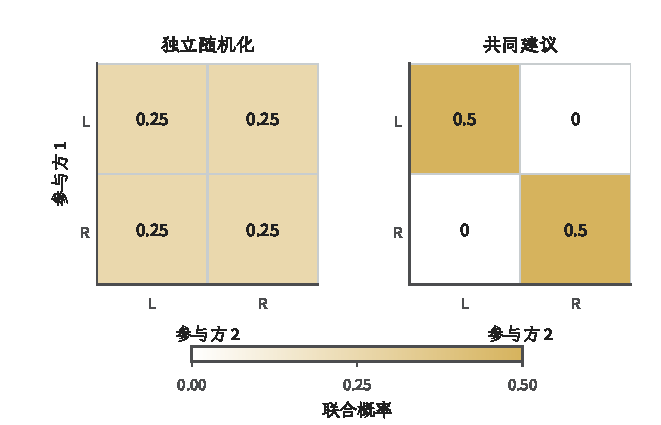
\includegraphics[width=\linewidth]{figures/math-preparation/concept-revision-dynamics/correlated-mass.pdf}
  \caption{二行动协调博弈的两个教学联合分布，共用$0$至$0.5$的概率色阶。
  行为参与者1的行动，列为参与者2的行动。左图为独立均匀策略，四格质量均为$0.25$；
  右图只推荐$(L,L)$与$(R,R)$，各占$0.5$。两者边缘概率均为$(0.5,0.5)$，
  但每人期望收益分别为$1$和$2$；相关分布并非边缘分布的乘积。}
  \label{fig:game-correlated-mass}
\end{figure}

\begin{table}[htbp]
  \centering
  \begin{tabular}{lcc}
    \toprule
    联合行动 & 独立混合概率 & 共同推荐概率\\
    \midrule
    $(L,L)$ & $1/4$ & $1/2$\\
    $(L,R)$ & $1/4$ & $0$\\
    $(R,L)$ & $1/4$ & $0$\\
    $(R,R)$ & $1/4$ & $1/2$\\
    \midrule
    每人的期望收益 & $1$ & $2$\\
    \bottomrule
  \end{tabular}
  \caption{同一边缘分布下的不同联合行动规律。教学协调博弈在相同行动时各得$2$，
  不同时各得$0$。右列是相关均衡，左列是独立混合Nash均衡；收益比较只针对这两个
  分布，纯策略协调均衡同样可以达到收益$2$。}
  \label{tab:game-independent-correlated-actions}
\end{table}

\section{按行动时可用的信息限制完整策略}
\label{sec:game-extensive-information}

收益矩阵将一套完整计划视为一个行动，但隐藏了行动顺序与当时可用的信息。
对三张牌博弈，看到自己牌面后的行动和看到对手质询后的行动不能依赖同一信息。
历史树记录先后关系，信息集把参与者无法区分的历史放在一起，从而限定策略能怎样实施。
这种信息限制独立于零和或一般和的收益分类，也决定下一节允许比较哪些策略偏离。

\subsection{历史树、机会节点与信息集}

\begin{definition}[有限扩展式博弈的历史树]
\label{def:game-finite-extensive-history}
\term{扩展式博弈}（extensive-form game）用历史树保留这些信息。记\(H\)为非空有限历史
集合，空历史为\(\varnothing\)。它满足前缀封闭：若一串行动属于\(H\)，删去末尾
若干行动所得的前缀仍属于\(H\)。不能再延长的历史组成终止集合\(Z\subset H\)。
若\(h\notin Z\)，可选行动集合\(A(h)\)规定合法后继\(ha\)，参与者函数\(P(h)\)
指出下一步由哪位参与者行动；机会节点记为\(P(h)=c\)，其行动概率
\(\sigma_c(a\mid h)\)已给定、非负且在\(A(h)\)上和为\(1\)。终止历史\(z\)为每位
参与者给出收益\(u_i(z)\)。对各参与者，还需指定下面的信息集划分，才能完整确定博弈。
\end{definition}

三张牌质询博弈的机会节点先选择\(H\)或\(L\)，概率各为\(1/2\)。参与者1看到牌面，
所以“拿到\(H\)”与“拿到\(L\)”属于两个不同决策位置。若他选择\(P\)，历史立即
终止；若选择\(B\)，参与者2行动。参与者2只看到“发生了质询”，无法区分历史
\((H,B)\)与\((L,B)\)。

对参与者\(i\)，记全部由其行动的非终止历史为
\[
  H_i=\{h\in H\setminus Z:P(h)=i\}.
\]
\begin{definition}[信息集]
\label{def:game-information-set}
参与者\(i\)的\term{信息集}（information set）族\(\mathcal{I}_i\)是\(H_i\)
的一个划分，每个信息集\(I\in\mathcal{I}_i\)收集参与者当时无法区分的决策历史。
同一信息集中的历史必须具有相同的合法行动集，记这个共同集合为
\(A(I)=A(h)\)，其中\(h\in I\)。
\end{definition}
否则参与者连“现在能做什么”都无法由观察确定。
牌面例子中，参与者2的信息集为
\[
  I_2=\{(H,B),(L,B)\},
\]
可选行动都是\(\{C,F\}\)。信息集不是状态的另一名称。第
~\ref{sec:decision-dynamic-programming}节中的Markov状态用于预测给定行动后的未来
分布；信息集描述当前参与者无法区分哪些历史。两个节点可以有相同物理状态，却因参与者
记得不同过去而属于不同信息集，也可以物理状态不同却因观察受限而位于同一信息集。
参与者\(i\)的纯策略必须为每个\(I\in\mathcal{I}_i\)指定一个
\(A(I)\)中的行动，包括均衡路径上不会到达的信息集；因此它是一份完整的应急计划，
而不只是实际走过路径上的动作序列。

表~\ref{tab:game-card-information}将同一个小博弈中“真实发生了什么”和“行动者
能区分什么”并列写出。参与者2在两条质询历史上必须用同一个$c$，因为他看到的数据
相同。若直接为高牌和低牌分别设置$c_H,c_L$，便改变了可用信息，得到另一个博弈，
即使收益函数没有改动也不能复用当前的均衡。

\begin{table*}[htbp]
  \centering
  \begin{tabularx}{\linewidth}{lXXX}
    \toprule
    行动者 & 真实决策历史 & 当时可区分的信息 & 合法行动规则\\
    \midrule
    参与者1 & 拿到$H$或拿到$L$ & 私人牌面可见，属于两个信息集 & 可分别选$b_H,b_L$\\
    参与者2 & $(H,B)$或$(L,B)$ & 只看到质询，属于同一信息集 & 两条历史共用应对概率$c$\\
    机会 & 初始发牌 & 已给定的环境随机化 & $P(H)=P(L)=1/2$，参与者不能选择\\
    \bottomrule
  \end{tabularx}
  \caption{三张牌教学博弈的信息约束。$b_H,b_L$为对应牌面上的质询概率，$c$为
  参与者2看到质询后的应对概率。这些行为策略记号将在下一小节正式使用。}
  \label{tab:game-card-information}
\end{table*}

\subsection{行为策略、混合策略与完全回忆}

\begin{definition}[行为策略]
\label{def:game-behavior-strategy}
参与者\(i\)的\term{行为策略}（behavior strategy）
\(\sigma_i(a\mid I)\)在每个信息集\(I\in\mathcal{I}_i\)上分别给出$A(I)$上的概率分布；
同一信息集中的所有历史必须使用同一分布。
\end{definition}
三张牌例子可写成三个数：
\[
  b_H=\sigma_1(B\mid I_H),\qquad
  b_L=\sigma_1(B\mid I_L),\qquad
  c=\sigma_2(C\mid I_2).
\]
第~\ref{sec:game-matrix-zero-sum-duality}节得到的均衡对应
\[
  b_H^\star=1,\qquad b_L^\star=\frac13,\qquad c^\star=\frac13.
\]

战略式中的混合策略是在游戏开始时随机抽取一个完整纯计划；行为策略则在每个信息集
到达时随机选择。二者在一般情形下并不等价。若参与者会忘记自己早先知道的牌或采取的
行动，开局抽取的同一个随机计划可以在多个时刻制造相关性，而独立的局部随机化未必能
复制这种相关性。

\begin{definition}[完全回忆]
\label{def:game-perfect-recall}
\term{完全回忆}（perfect recall）要求参与者在同一信息集内不能混淆自己过去获得的
信息和采取的行动。更具体地说，任意两个属于同一信息集的历史，沿途经过的该参与者
信息集序列及其本人行动序列必须相同；这里的过去序列只记录当前节点之前的本人决策。
\end{definition}

\begin{theorem}[Kuhn实现等价]
\label{thm:game-kuhn-equivalence}
在有限完全回忆扩展式博弈中，对任一参与者，任意混合策略都存在一个行为策略，使二者
面对任意固定的对手与机会策略时诱导相同的终止历史分布；任意行为策略也存在具有同样
性质的混合策略。
\end{theorem}

\begin{proof}
先从混合策略构造行为策略。设\(\mu_i\)是在有限纯策略集合上的分布。完全回忆保证
每个信息集\(I\)都有唯一的本人前缀
\[
  \rho_i(I)
  =
  \bigl((I_1,a_1),\ldots,(I_k,a_k)\bigr),
\]
即到达\(I\)以前本人依次经过的信息集和采取的行动；同一\(I\)中的所有历史共享这条
前缀。记\(E_I\)为纯策略与这条前缀一致的事件。若
\(\mu_i(E_I)>0\)，定义
\[
  \sigma_i(a\mid I)
  =
  \frac{
    \mu_i\bigl(E_I\cap\{s_i:s_i(I)=a\}\bigr)
  }{
    \mu_i(E_I)
  },
\]
其中\(s_i\)表示一项完整纯策略，事件\(s_i(I)=a\)表示它在当前信息集指定行动
\(a\)；若分母为零，
就在\(A(I)\)上任取一个分布。

沿任意终止历史依次考察参与者\(i\)的行动。链式法则表明，\(\mu_i\)抽取的完整计划
与这条本人行动序列一致的概率，等于上述各条件概率的乘积，也就是行为策略
\(\sigma_i\)沿该历史贡献的到达概率。对手与机会的路径概率在两种表示下相同，所以
每个终止历史的总概率相同。分母为零的信息集只位于\(\mu_i\)赋予零概率的本人前缀
之后，任意补全都不改变这一结论。

反过来，给定行为策略\(\sigma_i\)，在游戏开始前为每个信息集独立抽取一个行动，并
把全部抽取结果组成纯策略\(s_i\)。令
\[
  \mu_i(s_i)
  =
  \prod_{I\in\mathcal{I}_i}
  \sigma_i\bigl(s_i(I)\mid I\bigr).
\]
对任意终止历史，把未出现在该历史上的信息集行动求和后都得到因子\(1\)，剩余因子
恰是行为策略沿该历史的行动概率乘积。因此该混合策略面对任意对手与机会策略，也诱导
与原行为策略相同的终止历史分布。
\end{proof}

完全回忆不能省略。考虑一位参与者先在\(I_1\)选择\(L\)或\(R\)，随后到达同一个
信息集\(I_2\)，却忘记了刚才的选择，并在\(I_2\)选择\(l\)或\(r\)。混合策略可以
各以\(1/2\)抽取完整计划\((L,l)\)与\((R,r)\)，只产生\(Ll\)和\(Rr\)两条历史。
任何行为策略若让第一步的\(L,R\)都以正概率出现，且让第二步的\(l,r\)也都以正概率
出现，就还会以正概率产生\(Lr\)和\(Rl\)；若把某个概率设为零，又无法同时保留前两条
历史各\(1/2\)的概率。因此局部独立随机化不能复现混合计划中的跨时相关性。

牌面例子满足完全回忆。参与者1只行动一次，参与者2也只在一个信息集行动，不存在忘记
自身观察或动作的机会。矩阵混合
\((B,P)\)概率\(2/3\)、\((B,B)\)概率\(1/3\)，在高牌信息集总是选择\(B\)，在
低牌信息集以概率\(1/3\)选择\(B\)，正好得到上述行为策略。

\subsection{自身、对手与机会到达概率}

给定联合行为策略\(\bm{\sigma}\)，历史
\[
  h=(a_1,\ldots,a_k)
\]
的\term{到达概率}（reach probability）是沿路径各次行动概率之积。把机会也看作
固定策略，可以写成
\begin{equation}
  \pi^{\bm{\sigma}}(h)
  =
  \pi_i^{\bm{\sigma}}(h)
  \pi_{-i}^{\bm{\sigma}}(h),
  \label{eq:game-reach-factorization}
\end{equation}
其中\(\pi_i^{\bm{\sigma}}(h)\)只乘参与者\(i\)在路径上的行动概率，
\(\pi_{-i}^{\bm{\sigma}}(h)\)则乘其他参与者与机会的概率。这个分解不会声称两部分
随机变量独立；它只是把同一条路径上的乘积按行动者归组。

从历史\(h\)继续到终止历史\(z\)的条件路径概率记为
\(\pi^{\bm{\sigma}}(h,z)\)。
\begin{definition}[反事实价值]
\label{def:game-counterfactual-value}
给定上述联合行为策略及到达权重，参与者\(i\)在信息集\(I\)采取行动\(a\in A(I)\)的
\term{反事实价值}（counterfactual value）定义为
\begin{equation}
  v_i^{\bm{\sigma}}(I,a)
  =
  \sum_{h\in I}
  \pi_{-i}^{\bm{\sigma}}(h)
  \sum_{z\succeq ha}
  \pi^{\bm{\sigma}}(ha,z)u_i(z).
  \label{eq:game-counterfactual-action-value}
\end{equation}
信息集当前策略的反事实价值为
\begin{equation}
  v_i^{\bm{\sigma}}(I)
  =
  \sum_{a\in A(I)}
  \sigma_i(a\mid I)
  v_i^{\bm{\sigma}}(I,a).
  \label{eq:game-counterfactual-value}
\end{equation}

\end{definition}
式~\eqref{eq:game-counterfactual-action-value}保留对手和机会到达\(I\)的权重，
却去掉参与者\(i\)自己在到达\(I\)以前的概率。它在问：假设参与者\(i\)把自己送到
这个信息集，其他方和机会以当前方式到达各节点时，当前行动价值如何。去掉自身到达权重
使一个很少被当前自身策略访问的信息集仍能积累学习信号。

在均衡牌面策略下，参与者2的信息集包含高牌质询与低牌质询两个节点。对参与者2而言，
相应反事实到达权重为
\[
  \frac12 b_H^\star=\frac12,
  \qquad
  \frac12 b_L^\star=\frac16.
\]
若把它们归一化，得到到达信息集后的信念
\[
  \mathbb{P}(H\mid B)=\frac34,\qquad
  \mathbb{P}(L\mid B)=\frac14.
\]
在这组权重下，参与者2选择应对的反事实价值为
$\frac12(-2)+\frac16(2)=-\frac23$，退让的反事实价值为
$(\frac12+\frac16)(-1)=-\frac23$。除以总权重$2/3$后，两项条件期望收益都为$-1$。
局部是否偏好一个行动由同一比例缩放保持，但跨信息集求和必须保留原权重。
后验概率用于该信息集内的条件决策，反事实价值则保留未归一化权重，以便把不同信息集的
局部偏离加回整局收益。两者只差一个到达概率因子，却服务于不同推导。

\subsection{信息结构与策略可实施性}

参与者2不能规定“看到高牌质询时应对，看到低牌质询时退让”，因为两个历史位于同一
信息集。一个策略偏离必须对信息集中的所有节点采用同一行动分布。若额外公开牌面，
\(I_2\)会拆成两个单点信息集，允许偏离集合扩大，原均衡也随之改变。信息增加不只是
改善概率估计，它还改变可实施策略的定义域。

未以正概率到达的信息集会带来信念边界。Nash均衡检查完整策略中的单方偏离，但不要求
每个零概率信息集上的信念都由Bayes公式唯一决定。若要分析序贯理性，需要进一步规定
扰动、信念一致性或更精细的均衡概念。本章只保留后续遗憾分解所需的完全回忆和到达概率，
不把Nash存在性扩写成所有动态精炼结论。

这里的“反事实”也不同于第~\ref{chap:causal-inference}章的因果反事实。因果反事实
固定同一单位的外生背景，再替换结构方程中的行动；反事实价值则人为去掉某位参与者的
自身到达概率，以衡量信息集上的策略偏离。两者都讨论“没有实际发生的另一选择”，但
概率空间、固定对象和识别问题并不相同。

\section{用局部遗憾控制整局偏离与平均策略}
\label{sec:game-regret-cfr}

前面已明确可实施策略和允许偏离，均衡存在却没有给出参与者怎样学习策略。
遗憾把实际多轮收益与某个替代策略的收益比较，是对学习过程的评价。
先在普通行动集上建立累计界，再借助信息集和完全回忆分解扩展式博弈的偏离；
得到平均策略的保证时，仍要区分它与末次策略收敛。

\subsection{外部遗憾、内部遗憾与比较类}

\begin{definition}[外部遗憾]
\label{def:game-external-regret}
设行动集$A$非空且有限，同一参与者连续进行\(T\)轮决策。第\(t\)轮选择行动\(a_t\)，并面对损失函数
\(\ell_t:A\to\mathbb{R}\)。相对于事后最佳固定行动的
\term{外部遗憾}（external regret）为
\begin{equation}
  R_{\mathrm{ext}}^T
  =
  \max_{a\in A}
  \sum_{t=1}^{T}
  \bigl(\ell_t(a_t)-\ell_t(a)\bigr).
  \label{eq:game-external-regret}
\end{equation}
\end{definition}
若\(R_{\mathrm{ext}}^T/T\to0\)，平均每轮损失渐近不高于任何一个始终使用的固定
行动。比较对象不是每轮都知道\(\ell_t\)后重新选择的动态先知；后者通常能取得更小
损失，也需要额外的变化预算或可预测性假设。

\begin{definition}[内部遗憾]
\label{def:game-internal-regret}
在同一行动损失序列下，\term{内部遗憾}（internal regret）允许把每次实际选择\(a\)的轮次统一替换成另一
行动\(b\)：
\[
  R_{a\to b}^T
  =
  \sum_{t=1}^{T}
  \mathbb{I}\{a_t=a\}
  \bigl(\ell_t(a)-\ell_t(b)\bigr).
\]
对$(a,b)\in A\times A$分别计算上述量，最大正部称为该轮数下的内部遗憾。
\end{definition}
所有这类替换的正遗憾都很小，意味着参与者看到“原本要选\(a\)”这一信号后，也不愿
系统地改成\(b\)。这正对应相关均衡中依赖建议的偏离；外部遗憾只对应粗相关均衡中的
固定偏离。

\subsection{投影更新的累计遗憾界}

第~\ref{sec:opt-nonsmooth-proximal}节的投影不只用于离线优化，也能控制在线累计
损失\scite{math-zinkevich2003online}设\(C\subseteq\mathbb{R}^d\)为非空闭凸集，
直径至多为\(D\geq0\)，即对任意\(\bm{u},\bm{v}\in C\)都有
\(\lVert\bm{u}-\bm{v}\rVert_2\leq D\)。给定轮数\(T\geq1\)和步长\(\eta>0\)，
第\(t\)轮在选择
\(\bm{w}^{(t)}\in C\)后观察凸损失\(f_t\)，取次梯度
\(\bm{g}^{(t)}\in\partial f_t(\bm{w}^{(t)})\)，并假设
\(\lVert\bm{g}^{(t)}\rVert_2\leq G\)，其中\(G\geq0\)。在线投影次梯度更新为
\begin{equation}
  \bm{w}^{(t+1)}
  =
  \Pi_C\bigl(
    \bm{w}^{(t)}-\eta\bm{g}^{(t)}
  \bigr).
  \label{eq:game-online-projected-gradient}
\end{equation}

\begin{theorem}[在线投影次梯度的外部遗憾]
\label{thm:game-online-gradient-regret}
对任意比较点\(\bm{w}\in C\)，更新
\eqref{eq:game-online-projected-gradient}满足
\begin{equation}
  \sum_{t=1}^{T}
  \bigl(
    f_t(\bm{w}^{(t)})-f_t(\bm{w})
  \bigr)
  \leq
  \frac{D^2}{2\eta}
  +\frac{\eta G^2T}{2}.
  \label{eq:game-online-gradient-regret-bound}
\end{equation}
当\(D>0\)且\(G>0\)时，取\(\eta=D/(G\sqrt{T})\)，右侧为
\(DG\sqrt{T}\)。若\(D=0\)，则\(C\)只有一个点；若\(G=0\)，次梯度不等式说明
每轮差值都不大于零。两种退化情形的遗憾上界均为零，无需使用这个步长公式。
\end{theorem}

\begin{proof}
欧氏投影不会增加到任意可行点的距离，所以
\begin{align*}
  \lVert\bm{w}^{(t+1)}-\bm{w}\rVert_2^2
  &\leq
  \lVert
    \bm{w}^{(t)}-\eta\bm{g}^{(t)}-\bm{w}
  \rVert_2^2\\
  &=
  \lVert\bm{w}^{(t)}-\bm{w}\rVert_2^2
  -2\eta
  \langle
    \bm{g}^{(t)},\bm{w}^{(t)}-\bm{w}
  \rangle
  +\eta^2\lVert\bm{g}^{(t)}\rVert_2^2.
\end{align*}
凸函数的次梯度不等式给出
\[
  f_t(\bm{w}^{(t)})-f_t(\bm{w})
  \leq
  \langle
    \bm{g}^{(t)},\bm{w}^{(t)}-\bm{w}
  \rangle.
\]
把内积从距离展开式中解出并代入，得到
\[
  f_t(\bm{w}^{(t)})-f_t(\bm{w})
  \leq
  \frac{
    \lVert\bm{w}^{(t)}-\bm{w}\rVert_2^2
    -
    \lVert\bm{w}^{(t+1)}-\bm{w}\rVert_2^2
  }{2\eta}
  +\frac{\eta G^2}{2}.
\]
对\(t\)求和后，距离平方项望远镜消去，只剩初始距离上界\(D^2\)，得到
式~\eqref{eq:game-online-gradient-regret-bound}。当\(D,G>0\)时，对右侧关于
\(\eta\)配平即得\(DG\sqrt{T}\)；退化情形按定理后的说明处理。
\end{proof}

这个证明允许损失序列依赖过去行动，只要当前行动在当前损失揭晓前确定。它给出
\(O(\sqrt{T})\)累计遗憾和\(O(T^{-1/2})\)平均遗憾，却没有声称
\(\bm{w}^{(t)}\)本身收敛。把低遗憾用于博弈时，通常得到经验分布或平均策略的结论。

概率单纯形把这个通用更新接回混合策略。设行动集为
\(A=\{B,P\}\)，取\(C=\Delta(A)\)，并令第\(t\)轮两个行动的损失向量为
\(\bm{\ell}^{(t)}\)。分布\(\bm{w}\in C\)的期望损失
\[
  f_t(\bm{w})
  =
  \langle\bm{w},\bm{\ell}^{(t)}\rangle
\]
是线性函数，次梯度就是\(\bm{\ell}^{(t)}\)。若
\(\bm{w}^{(t)}=(1/2,1/2)^{\top}\)、
\(\bm{\ell}^{(t)}=(0,1)^{\top}\)且\(\eta=1/2\)，则
\[
  \Pi_{\Delta(A)}
  \left(
    \bm{w}^{(t)}-\eta\bm{\ell}^{(t)}
  \right)
  =
  (3/4,1/4)^{\top}.
\]
投影把概率从本轮损失较大的\(P\)移向\(B\)，同时保持坐标非负且和为\(1\)。
定理因而说明混合策略空间上可以构造局部无外部遗憾更新。下面的CFR在各信息集采用
遗憾匹配，而不是必须采用欧氏投影；这里的通用结果用于建立两类更新共享的无遗憾目标。

\subsection{信息集上的即时反事实遗憾}

前两小节采用损失约定，遗憾写成实际损失减替代损失。扩展式博弈沿用收益函数，下面改用
收益约定，把遗憾写成替代收益减当前收益；令损失等于收益的相反数，就能在两种约定之间
转换，正遗憾始终表示偏离更有利。

在第\(t\)轮扩展式博弈中，联合策略记为\(\bm{\sigma}^{(t)}\)。参与者\(i\)在信息集
\(I\)把当前随机行动改成固定行动\(a\)的即时反事实遗憾为
\begin{equation}
  r_i^{(t)}(I,a)
  =
  v_i^{\bm{\sigma}^{(t)}}(I,a)
  -
  v_i^{\bm{\sigma}^{(t)}}(I).
  \label{eq:game-immediate-counterfactual-regret}
\end{equation}
累计量及其正部最大值记为
\[
  R_i^T(I,a)
  =
  \sum_{t=1}^{T}r_i^{(t)}(I,a),
  \qquad
  R_{i,+}^T(I)
  =
  \max\left\{0,\max_{a\in A(I)}R_i^T(I,a)\right\}.
\]

\term{反事实遗憾最小化}（counterfactual regret minimization, CFR）在每个信息集
运行一个局部无遗憾算法\scite{math-zinkevich2007cfr}一次完整树更新包含四步：
固定本轮联合行为策略并遍历历史树，计算各信息集的反事实行动价值；用
式~\eqref{eq:game-immediate-counterfactual-regret}累计每个行动的遗憾；用局部
遗憾匹配生成下一轮策略；同时按本人的到达概率累计平均策略所需的实现权重。这里的
“最小化”是让平均遗憾趋近于零，不是逐轮直接最小化某个静态目标。

典型的\term{遗憾匹配}（regret matching）按正累计遗憾选择下一轮行动：
\begin{equation}
  \sigma_i^{(t+1)}(a\mid I)
  =
  \begin{cases}
    \displaystyle
    \frac{[R_i^t(I,a)]_+}
         {\sum_b[R_i^t(I,b)]_+},
      &\sum_b[R_i^t(I,b)]_+>0,\\[8pt]
    \displaystyle\frac{1}{|A(I)|},
      &\text{否则}.
  \end{cases}
  \label{eq:game-regret-matching}
\end{equation}

若存在\(\Delta_I\geq0\)，使对每轮\(t=1,\ldots,T\)及任意
\(a,b\in A(I)\)都有
\[
  \left|
    v_i^{\bm{\sigma}^{(t)}}(I,a)
    -
    v_i^{\bm{\sigma}^{(t)}}(I,b)
  \right|
  \leq\Delta_I,
\]
则遗憾匹配满足
\begin{equation}
  R_{i,+}^T(I)
  \leq
  \Delta_I\sqrt{|A(I)|T}.
  \label{eq:game-local-regret-matching-bound}
\end{equation}
证明可用势函数
\(\Phi_t=\sum_a[R_i^t(I,a)]_+^2\)。每轮平方展开中的交叉项为
\[
  2\sum_a[R_i^{t-1}(I,a)]_+r_i^{(t)}(I,a).
\]
当正遗憾和非零时，式~\eqref{eq:game-regret-matching}使它正比于
\(\sum_a\sigma_i^{(t)}(a\mid I)r_i^{(t)}(I,a)=0\)；正遗憾和为零时，
交叉项也不为正。平方增量至多
\(\sum_a(r_i^{(t)}(I,a))^2\leq |A(I)|\Delta_I^2\)。
归纳得到
\(\Phi_T\leq T|A(I)|\Delta_I^2\)，而每个正累计遗憾的平方不超过
\(\Phi_T\)，于是得到式~\eqref{eq:game-local-regret-matching-bound}。

\subsection{牌面博弈的反事实遗憾计算}

用三张牌博弈核对一次参与者2的CFR更新。假设当前策略取
\[
  b_H=b_L=\frac12,\qquad
  \sigma_2(C\mid I_2)=\sigma_2(F\mid I_2)=\frac12.
\]
参与者2到达高牌质询节点和低牌质询节点的反事实权重都为
\[
  \frac12\cdot\frac12=\frac14.
\]
第一个因子来自机会发牌，第二个因子来自参与者1质询。应对
\(C\)时，参与者2在高牌和低牌节点的收益分别为\(-2\)与\(2\)，所以
\[
  v_2(I_2,C)
  =
  \frac14(-2)+\frac14(2)=0.
\]
退让\(F\)时，参与者1在两个节点都得到\(1\)，参与者2因而都得到\(-1\)，所以
\[
  v_2(I_2,F)
  =
  \frac14(-1)+\frac14(-1)=-\frac12.
\]
当前均匀策略的反事实价值为\(-1/4\)，本轮即时遗憾因此为
\[
  r_2(I_2,C)=\frac14,\qquad
  r_2(I_2,F)=-\frac14.
\]
若此前累计遗憾为零，遗憾匹配在下一轮把全部概率放到\(C\)。这个结果只描述一次局部
更新；参与者2更常应对以后，低牌质询会变得不利，参与者1的后续更新又会改变两个节点的
权重。因而不能把首轮纯响应当成收敛策略，也不能从这一个数值步骤推出均衡保证。

\subsection{完全回忆与局部遗憾分解}

整局外部遗憾允许参与者把当前行为策略替换成任意固定行为策略：
\begin{equation}
  R_i^T
  =
  \max_{\widetilde{\sigma}_i}
  \sum_{t=1}^{T}
  \left[
    u_i(\widetilde{\sigma}_i,\bm{\sigma}_{-i}^{(t)})
    -
    u_i(\bm{\sigma}^{(t)})
  \right].
  \label{eq:game-extensive-external-regret}
\end{equation}
局部反事实遗憾之所以有用，在于它们能够上界这个看似覆盖整棵树的比较。

\begin{theorem}[CFR的反事实遗憾分解]
\label{thm:game-cfr-decomposition}
在有限完全回忆扩展式博弈中，
\begin{equation}
  R_i^T
  \leq
  \sum_{I\in\mathcal{I}_i}
  R_{i,+}^T(I).
  \label{eq:game-cfr-global-bound}
\end{equation}
\end{theorem}

\begin{proof}
固定替代行为策略\(\widetilde{\sigma}_i\)。证明先在一轮中把整局偏离逐层拆开，再对
轮次求和。为看清拆分发生在哪里，对\(h\in I\)定义当前策略在行动\(a\)后的条件续局
收益
\[
  q_i^{(t)}(h,a)
  =
  \sum_{z\succeq ha}
  \pi^{\bm{\sigma}^{(t)}}(ha,z)u_i(z),
\]
并以\(\widetilde q_i^{(t)}(h,a)\)表示对手和机会仍采用
\(\bm{\sigma}_{-i}^{(t)}\)，而参与者\(i\)从\(ha\)以后采用
\(\widetilde{\sigma}_i\)时的同一数值，即
\[
  \widetilde q_i^{(t)}(h,a)
  =
  \sum_{z\succeq ha}
  \pi^{(\widetilde{\sigma}_i,\bm{\sigma}_{-i}^{(t)})}(ha,z)
  u_i(z).
\]
当前策略从\(h\)出发的续局收益为
\(q_i^{(t)}(h)=\sum_b\sigma_i^{(t)}(b\mid I)q_i^{(t)}(h,b)\)。
在替代收益中加上再减去“只在当前行动改用替代分布、以后仍用当前策略”的收益，逐历史
得到恒等式
\begin{align}
  &\sum_{a\in A(I)}
  \widetilde{\sigma}_i(a\mid I)
  \widetilde q_i^{(t)}(h,a)
  -
  q_i^{(t)}(h)
  \notag\\
  &\quad=
  \sum_{a\in A(I)}
  \widetilde{\sigma}_i(a\mid I)
  \bigl(q_i^{(t)}(h,a)-q_i^{(t)}(h)\bigr)
  \notag\\
  &\qquad\quad+
  \sum_{a\in A(I)}
  \widetilde{\sigma}_i(a\mid I)
  \bigl(
    \widetilde q_i^{(t)}(h,a)-q_i^{(t)}(h,a)
  \bigr).
  \label{eq:game-history-deviation-identity}
\end{align}
第一项只改变当前信息集的行动，第二项只记录当前行动之后继续偏离的收益。

下面把逐历史恒等式汇总到信息集。记
\(\mathcal{C}_i(I,a)\)为采取\(a\)以后、在参与者\(i\)再次行动时首次遇到的本人
信息集集合；若在此之前终止，就没有后继信息集。令
\(\widetilde v_i^{(t)}(I)\)为到达\(I\)的对手与机会权重仍取
\(\pi_{-i}^{\bm{\sigma}^{(t)}}(h)\)，但从\(I\)起参与者\(i\)都采用
\(\widetilde{\sigma}_i\)的反事实价值，并记
\[
  D_i^{(t)}(I)
  =
  \widetilde v_i^{(t)}(I)
  -
  v_i^{\bm{\sigma}^{(t)}}(I),
  \qquad
  L_i^{(t)}(I)
  =
  \sum_a
  \widetilde{\sigma}_i(a\mid I)r_i^{(t)}(I,a).
\]
将式~\eqref{eq:game-history-deviation-identity}乘以
\(\pi_{-i}^{\bm{\sigma}^{(t)}}(h)\)并对\(h\in I\)求和，得到信息集偏离收益恒等式
\begin{equation}
  D_i^{(t)}(I)
  =
  L_i^{(t)}(I)
  +
  \sum_{a\in A(I)}
  \widetilde{\sigma}_i(a\mid I)
  \sum_{I'\in\mathcal{C}_i(I,a)}
  D_i^{(t)}(I').
  \label{eq:game-information-set-deviation-identity}
\end{equation}
这里没有漏掉从\(I\)到\(I'\)之间的概率：这段路径上参与者\(i\)不再行动，对手和
机会的路径概率与\(I\)处已有的权重相乘，正好成为\(I'\)中各历史的
\(\pi_{-i}^{\bm{\sigma}^{(t)}}\)。在遇到下一个本人信息集以前终止的路径上，两种
策略的后续行为相同，故其第二项为零。

完全回忆使本人信息集及边\((I,a)\to I'\)组成一个森林。确切地说，同一信息集
\(I'\)中的所有历史具有相同的本人既往信息集与行动序列，所以每个非根信息集都有唯一的
前驱边；对手或机会的多条历史可以汇入同一个\(I'\)，但这些历史只在
\(\pi_{-i}^{\bm{\sigma}^{(t)}}\)的求和中合并，不会把\(I'\)复制成多个后继。
记\(\widetilde{\pi}_i(I)\)为替代策略沿该唯一本人前缀的行动概率乘积；根信息集的
乘积约定为\(1\)。这正是反事实价值中故意省去的自身到达概率。

现在按一个信息集之后还可能遇到的本人信息集层数归纳。最深信息集没有后继，
式~\eqref{eq:game-information-set-deviation-identity}给出
\(D_i^{(t)}(I)=L_i^{(t)}(I)\)。假设所有深度更小的后继子树都已展开，把它们代回
同一恒等式；由于每个后继只有一个前驱，子树中的每个信息集恰好出现一次，其系数等于
沿唯一前缀的\(\widetilde{\sigma}_i\)行动概率乘积。对森林的所有根求和后便得到
\begin{equation}
  u_i(\widetilde{\sigma}_i,\bm{\sigma}_{-i}^{(t)})
  -
  u_i(\bm{\sigma}^{(t)})
  =
  \sum_{I\in\mathcal{I}_i}
  \widetilde{\pi}_i(I)
  \sum_{a\in A(I)}
  \widetilde{\sigma}_i(a\mid I)r_i^{(t)}(I,a).
  \label{eq:game-global-deviation-identity}
\end{equation}
参与者\(i\)从未行动就终止的历史在两种策略下收益相同，因而不出现在右侧。
式~\eqref{eq:game-global-deviation-identity}明确分开了两类权重：对手与机会的权重
已经包含在\(r_i^{(t)}(I,a)\)中，自身在替代策略下到达\(I\)的权重则是外部系数
\(\widetilde{\pi}_i(I)\)。

替代策略固定后，\(\widetilde{\pi}_i(I)\)和
\(\widetilde{\sigma}_i(a\mid I)\)都不随\(t\)变化。对
式~\eqref{eq:game-global-deviation-identity}求和，并使用
\(0\leq\widetilde{\pi}_i(I)\leq1\)，可得
\begin{align*}
  &\sum_{t=1}^{T}
  \left[
    u_i(\widetilde{\sigma}_i,\bm{\sigma}_{-i}^{(t)})
    -
    u_i(\bm{\sigma}^{(t)})
  \right]\\
  &\quad=
  \sum_I
  \widetilde{\pi}_i(I)
  \sum_a
  \widetilde{\sigma}_i(a\mid I)R_i^T(I,a)\\
  &\quad\leq
  \sum_I
  \widetilde{\pi}_i(I)
  \max_a R_i^T(I,a)
  \leq
  \sum_I R_{i,+}^T(I).
\end{align*}
最后一个不等式也覆盖\(\max_aR_i^T(I,a)<0\)的情形，因为此时相应正部为零。
右侧与替代策略无关，再对\(\widetilde{\sigma}_i\)取最大，就得到
式~\eqref{eq:game-cfr-global-bound}。
\end{proof}

若缺少完全回忆，同一当前信息集可能汇合不同的本人行动历史。此时局部策略无法知道应该
补回哪条自身到达路径，上述递归可能重复计算或遗漏偏离收益，局部低遗憾便不再自动控制
整局外部遗憾。

结合式~\eqref{eq:game-local-regret-matching-bound}，CFR得到
\begin{equation}
  R_i^T
  \leq
  \sum_{I\in\mathcal{I}_i}
  \Delta_I\sqrt{|A(I)|T}.
  \label{eq:game-cfr-rate}
\end{equation}
当信息集和行动数固定时，平均外部遗憾按\(O(T^{-1/2})\)趋于零。

\subsection{平均策略的权重与零和保证}

行为策略不能在每个信息集直接做普通算术平均。某轮中一个信息集若几乎不会被参与者自己
到达，该处局部概率不应与频繁到达轮次具有同样权重。完全回忆保证同一信息集
\(I\)中的历史具有同一条本人行动前缀，因而
\(\pi_i^{\bm{\sigma}^{(t)}}(I)\)定义为这条前缀上的本人行动概率乘积，与选取
哪个\(h\in I\)无关。记第\(t\)轮在本人序列\((I,a)\)上的实现权重为
\[
  x_i^{(t)}(I,a)
  =
  \pi_i^{\bm{\sigma}^{(t)}}(I)
  \sigma_i^{(t)}(a\mid I),
\]
并令
\(\overline{x}_i^T(I,a)=T^{-1}\sum_t x_i^{(t)}(I,a)\)以及
\(\overline{x}_i^T(I)=T^{-1}\sum_t
\pi_i^{\bm{\sigma}^{(t)}}(I)\)。CFR使用
\begin{equation}
  \overline{\sigma}_i^T(a\mid I)
  =
  \frac{
    \sum_{t=1}^{T}
    \pi_i^{\bm{\sigma}^{(t)}}(I)
    \sigma_i^{(t)}(a\mid I)
  }{
    \sum_{t=1}^{T}
    \pi_i^{\bm{\sigma}^{(t)}}(I)
  },
  \label{eq:game-cfr-average-strategy}
\end{equation}
其中分母为零时可以任意指定。式~\eqref{eq:game-cfr-average-strategy}等价于
\[
  \overline{\sigma}_i^T(a\mid I)
  =
  \frac{\overline{x}_i^T(I,a)}{\overline{x}_i^T(I)}.
\]

这个权重不是经验修正，而是实现计划平均所要求的条件概率。根本人序列的实现权重为
\(1\)。若\(I\)的唯一本人前驱序列终止于\((J,b)\)，则每一轮都有
\(\pi_i^{\bm{\sigma}^{(t)}}(I)=x_i^{(t)}(J,b)\)，对轮次平均后仍有
\(\overline{x}_i^T(I)=\overline{x}_i^T(J,b)\)。从根序列归纳，并在每个信息集应用
上面的条件概率公式，得到
\begin{equation}
  \pi_i^{\overline{\sigma}_i^T}(I)
  \overline{\sigma}_i^T(a\mid I)
  =
  \overline{x}_i^T(I,a)
  =
  \frac{1}{T}\sum_{t=1}^{T}x_i^{(t)}(I,a).
  \label{eq:game-average-realization-plan}
\end{equation}
因此，加权平均行为策略实现的正是各轮本人实现计划的算术平均。分母为零意味着所有轮次
到达该本人序列的概率都为零，此处怎样指定局部策略都不改变平均实现计划。

在两人零和博弈中，若双方平均外部遗憾分别不超过
\(\varepsilon_1T\)与\(\varepsilon_2T\)，则平均策略满足
\begin{equation}
  \max_{\sigma_1}
  u_1(\sigma_1,\overline{\sigma}_2^T)
  -
  \min_{\sigma_2}
  u_1(\overline{\sigma}_1^T,\sigma_2)
  \leq
  \varepsilon_1+\varepsilon_2.
  \label{eq:game-average-exploitability}
\end{equation}
下面补出这个界。记第\(t\)轮第1位参与者的收益为
\(u_1(\sigma_1^{(t)},\sigma_2^{(t)})\)，并令
\[
  \widehat u_T
  =
  \frac{1}{T}
  \sum_{t=1}^{T}
  u_1(\sigma_1^{(t)},\sigma_2^{(t)}).
\]
终止历史\(z\)的概率可以写成机会概率与双方实现权重之积，所以期望收益对双方实现计划
分别线性。结合式~\eqref{eq:game-average-realization-plan}，对任意固定策略
\(\sigma_1,\sigma_2\)有
\begin{align}
  \frac{1}{T}\sum_{t=1}^{T}
  u_1(\sigma_1,\sigma_2^{(t)})
  &=
  u_1(\sigma_1,\overline{\sigma}_2^T),
  \notag\\
  \frac{1}{T}\sum_{t=1}^{T}
  u_1(\sigma_1^{(t)},\sigma_2)
  &=
  u_1(\overline{\sigma}_1^T,\sigma_2).
  \label{eq:game-average-payoff-linearity}
\end{align}

第1位参与者的外部遗憾界除以\(T\)，再用第一条等式，得到
\begin{equation}
  \max_{\sigma_1}
  u_1(\sigma_1,\overline{\sigma}_2^T)
  -
  \widehat u_T
  \leq
  \varepsilon_1.
  \label{eq:game-row-average-regret}
\end{equation}
第2位参与者的收益为\(u_2=-u_1\)。把其外部遗憾界同样除以\(T\)，并用
式~\eqref{eq:game-average-payoff-linearity}的第二条等式，得到
\begin{equation}
  \widehat u_T
  -
  \min_{\sigma_2}
  u_1(\overline{\sigma}_1^T,\sigma_2)
  \leq
  \varepsilon_2.
  \label{eq:game-column-average-regret}
\end{equation}
将式~\eqref{eq:game-row-average-regret}与
\eqref{eq:game-column-average-regret}相加，经验对局收益
\(\widehat u_T\)消去，正好得到
式~\eqref{eq:game-average-exploitability}。若博弈值为\(v^\star\)，其左侧还可写成
\[
  \left[
    \max_{\sigma_1}u_1(\sigma_1,\overline{\sigma}_2^T)-v^\star
  \right]
  +
  \left[
    v^\star-\min_{\sigma_2}u_1(\overline{\sigma}_1^T,\sigma_2)
  \right].
\]
两项分别衡量第2位和第1位参与者的平均策略可被最佳响应利用多少，且都非负；因此该和是
双方平均策略的零和鞍点间隙。本章把这个和称为\term{联合可利用度}
（joint exploitability）；若采用两项平均的口径，数值还需除以\(2\)。间隙为零时，
两者构成极小极大策略对。

式~\eqref{eq:game-average-exploitability}保证的是两人零和博弈的平均策略，不是最后
一次迭代。一般和博弈中，低外部遗憾使经验联合分布趋近CCE，却不保证平均边缘策略构成
Nash均衡。为看清这里保留的是哪种分布，令第\(t\)轮实际联合行动为
\(\bm{a}^{(t)}\)，经验分布为
\[
  \widehat{\mu}_T(\bm{a})
  =
  \frac{1}{T}
  \sum_{t=1}^{T}
  \mathbb{I}\{\bm{a}^{(t)}=\bm{a}\}.
\]
若参与者\(i\)的平均外部收益遗憾至多\(\varepsilon_i\)，则对任意固定行动
\(a_i'\)，
\[
  \mathbb{E}_{\bm{A}\sim\widehat{\mu}_T}[u_i(\bm{A})]
  \geq
  \mathbb{E}_{\bm{A}\sim\widehat{\mu}_T}
  [u_i(a_i',\bm{A}_{-i})]
  -\varepsilon_i.
\]
这正是带\(\varepsilon_i\)松弛的CCE不等式。若每个有向替换
\(a_i\to b_i\)的平均内部遗憾都不超过\(\varepsilon_i\)，则对任意映射
\(\phi_i\)，把发生\(A_i=a_i\)的轮次按\(a_i\)分组并求和，可得CE偏离收益至多
\(|A_i|\varepsilon_i\)；若直接控制所有映射的交换遗憾，则松弛就是
\(\varepsilon_i\)。这两个结论保留的是联合经验分布中的相关性，不能用各自经验边缘
的乘积替代。

末次策略还可能持续循环。采样CFR若只访问部分历史，还要用第
\ref{chap:stochastic-processes-and-approximation}章的无偏估计、方差和集中工具控制
采样误差，不能把完整树上的确定性分解直接当作有限样本保证。

回到三张牌例子，参与者2的信息集使用高牌质询权重\(1/2\)和低牌质询权重\(1/6\)
计算局部应对遗憾。若算法长期发现应对比退让更好，就提高\(C\)的概率；这一变化又会
降低低牌质询的收益，使参与者1减少虚张声势。双方局部更新相互改变下一轮价值，CFR保证
累计偏离受控，却不要求这两个概率逐轮单调走向\(1/3\)。

把平均遗憾转成均衡结论时，还要保留产生平均的联合样本。
表~\ref{tab:game-regret-comparison-conclusions}比较两种偏离：固定行动只提出一个
事前替代选择，内部替换可以对某种已采取行动单独修改，因此后者需要控制更多比较。
这里的保证针对经验联合分布或相应的平均策略，不对最后一轮作同样承诺。

\begin{table*}[htbp]
  \centering
  \begin{tabularx}{\linewidth}{lXXX}
    \toprule
    偏离比较 & 允许怎样改变 & 一般和下的平均结论 & 两人零和的补充\\
    \midrule
    外部遗憾 & 所有轮次统一改用一个固定行动 & 经验联合分布的粗相关偏离收益小 & 双方平均策略的鞍点差距小\\
    内部遗憾 & 将某种已选行动统一换成另一行动 & 经验联合分布的相关偏离收益小 & 仍需按具体信息结构恢复策略\\
    \bottomrule
  \end{tabularx}
  \caption{遗憾的比较类与平均结论。表中要求每位参与者都控制相应的平均遗憾；
  扩展式博弈的平均行为策略还须使用自身到达权重。末次策略收敛不由这些平均结论推出。}
  \label{tab:game-regret-comparison-conclusions}
\end{table*}

\section{按贡献、退出条件与联盟稳定性分配收益}
\label{sec:game-credit-allocation-multiparty-payoffs}

遗憾与均衡研究参与者各自选择策略。若任务改为合作，并已给出每个联盟能够取得的价值，
问题就变成共同收益怎样分配。边际贡献取决于加入顺序，Shapley值对这些顺序作平均；
联盟是否愿意保持合作则是另一个稳定性要求，需要与分配公平的公理分别核对。

\subsection{联盟价值、边际贡献与分配}

前四节把参与者的收益函数视为已给定对象。合作问题进一步询问：若若干参与者共享信息、
模型或资源并产生共同收益，这个收益应怎样分配？本节所说的
\term{多方信用分配}（multi-party credit allocation），是根据各个联盟能够取得的
价值，为每位参与者确定贡献份额\(\psi_i(v)\)。若还要求预算平衡，则这些份额满足
\(\sum_i\psi_i(v)=v(N)\)。它分配的是参与者对联盟价值的贡献，不是把一条轨迹的
延迟奖励传回各时间步；后者将在强化学习部分作为时序信用分配问题讨论。

\begin{definition}[可转移效用博弈]
\label{def:game-transferable-utility-cooperation}
\term{可转移效用合作博弈}
（transferable-utility cooperative game）由参与者集合\(N\)和联盟价值函数
\[
  v:2^N\to\mathbb{R},\qquad v(\varnothing)=0
\]
组成，$N$为非空有限集合。\(v(S)\)表示联盟\(S\)独立合作时可取得并能在成员之间转移的总收益。
\end{definition}

联盟价值不是从单个模型输出自动得到的。对牌面判断任务，可以把\(v(S)\)定义为联盟
\(S\)共享信号后，相对于无信号基线减少的最优期望损失；也可以定义为收入、正确判断数
或节省的核验成本。不同定义会产生不同分配。若参与者的收益不能用同一尺度转移，例如
一方关心隐私、另一方关心延迟，就需要非可转移效用模型，不能先相加再假装总量可任意
拆分。

参与者\(i\)加入已有联盟\(S\subseteq N\setminus\{i\}\)的边际贡献为
\[
  v(S\cup\{i\})-v(S).
\]
它依赖先到者集合\(S\)。两位牌面观察者可能各自只能提供模糊线索，合在一起却能确定
牌面；此时任何一人的“独立贡献”都不能由单独使用他的信号一次决定。

\subsection{Shapley值与参与顺序平均}

\term{Shapley值}（Shapley value）把参与者在所有随机加入次序中的边际贡献取平均
\scite{math-shapley1953value}
\begin{definition}[Shapley值]
\label{def:game-shapley-value}
对上述可转移效用博弈、\(n=|N|\)及参与者$i\in N$，其Shapley分配为
\begin{equation}
  \phi_i(v)
  =
  \sum_{S\subseteq N\setminus\{i\}}
  \frac{|S|!(n-|S|-1)!}{n!}
  \bigl[
    v(S\cup\{i\})-v(S)
  \bigr].
  \label{eq:game-shapley-value}
\end{equation}
\end{definition}
系数是随机排列中恰好由\(S\)排在\(i\)之前的概率：\(S\)内部有\(|S|!\)种次序，
其余参与者在\(i\)之后有\((n-|S|-1)!\)种次序，总排列数为\(n!\)。

Shapley值满足四项要求。若两位参与者对所有不含二者的联盟产生相同边际贡献，
\term{对称性}要求二者分配相同；若参与者对任意联盟的边际贡献都为零，
\term{虚设参与者性质}要求其分配为零；\term{有效性}要求
\(\sum_i\phi_i(v)=v(N)\)；\term{可加性}要求对两个价值函数
\(v,w\)，有\(\phi_i(v+w)=\phi_i(v)+\phi_i(w)\)。

\begin{theorem}[Shapley值的公理刻画]
\label{thm:game-shapley-characterization}
在有限可转移效用合作博弈上，同时满足对称性、虚设参与者性质、有效性和可加性的分配
规则唯一，并由式~\eqref{eq:game-shapley-value}给出。
\end{theorem}

\begin{proof}
先验证式~\eqref{eq:game-shapley-value}满足四项性质。它是随机排列下边际贡献的期望。
每个排列中，所有参与者的边际贡献沿加入次序望远镜相加为
\[
  v(N)-v(\varnothing)=v(N),
\]
取期望得到有效性。交换两位对称参与者不会改变排列分布或边际贡献分布，得到对称性。
虚设参与者的每项边际贡献都为零。边际贡献关于价值函数线性，取期望后得到可加性。

再证唯一性。设\(\Phi\)是任意满足四项公理的分配规则。对每个非空集合
\(T\subseteq N\)，定义一致联盟博弈
\[
  u_T(S)
  =
  \begin{cases}
    1,&T\subseteq S,\\
    0,&T\nsubseteq S.
  \end{cases}
\]
任意满足\(v(\varnothing)=0\)的价值函数都能唯一写成
\begin{equation}
  v
  =
  \sum_{\varnothing\neq T\subseteq N}
  c_Tu_T,
  \qquad
  c_T
  =
  \sum_{R\subseteq T}
  (-1)^{|T|-|R|}v(R),
  \label{eq:game-unanimity-basis}
\end{equation}
这是子集格上的包含--排除展开。

还要处理展开式中的任意实系数，不能只由重复相加得到整数或有理数倍。对任意
\(c\in\mathbb{R}\)，在博弈\(c\,u_T\)中，\(T\)外的参与者都是虚设参与者，分配
必须为零；\(T\)内参与者彼此对称，有效性又要求他们的分配和为\(c\)，所以每人只能
得到\(c/|T|\)。这个结论直接覆盖正、负及无理的\(c\)，没有预先假设分配规则连续。

式~\eqref{eq:game-unanimity-basis}只有有限项。可加性因此给出
\[
  \Phi(v)
  =
  \sum_{\varnothing\neq T\subseteq N}
  \Phi(c_Tu_T),
\]
而每一项已经由上一段唯一确定，故任意\(v\)上的分配也唯一。特别地，对任意
\(\alpha\in\mathbb{R}\)，对\(\alpha v\)使用同一展开便得到
\(\Phi(\alpha v)=\alpha\Phi(v)\)，这补出了实齐次性。前半部分已经证明
式~\eqref{eq:game-shapley-value}满足这些公理，故它就是唯一规则。
\end{proof}

\subsection{三方信息合作的贡献分配}

把牌面任务扩展为三位信息提供者。参与者1观察牌背纹理，参与者2观察发牌动作，
参与者3提供一次较弱的设备校验。以“相对于无信息基线减少的期望损失”为统一收益单位，
假设教学构造的联盟价值为
\[
\begin{array}{c@{\quad}cccccccc}
  S
  &\varnothing&\{1\}&\{2\}&\{3\}
  &\{1,2\}&\{1,3\}&\{2,3\}&\{1,2,3\}\\ \hline
  v(S)
  &0&1&1&0&3&2&2&4
\end{array}
\]
这些数值只用于展示互补贡献：前两位各自有用，二者合并额外增益较大；第三位单独无用，
却能校验已有线索。

对参与者1，四类前驱联盟的贡献给出
\begin{align*}
  \phi_1(v)
  &=
  \frac13(1-0)
  +\frac16(3-1)
  +\frac16(2-0)
  +\frac13(4-2)\\
  &=\frac53.
\end{align*}
对称性给出\(\phi_2(v)=5/3\)。参与者3的分配为
\begin{align*}
  \phi_3(v)
  &=
  \frac13(0-0)
  +\frac16(2-1)
  +\frac16(2-1)
  +\frac13(4-3)\\
  &=\frac23.
\end{align*}
三者之和为\(4=v(N)\)，与有效性一致。参与者3虽然单独价值为零，却不是虚设参与者，
因为加入\(\{1\}\)、\(\{2\}\)或\(\{1,2\}\)都会增加联盟价值。只按单人表现分配会
漏掉这种互补性。

若把价值改成模型预测分数，Shapley公式仍可计算，但解释也随之改变。它分配的是所定义
价值函数相对于基线的差，不自动等于真实因果贡献。特征彼此相关时，“缺少某个特征”的
联盟输入怎样构造还需要条件分布、边缘分布或干预语义；这些选择分别回答预测归因与因果
效应问题，不能只用同一个Shapley名称消除差异。

\subsection{联盟稳定性、Pareto权衡与协商解}

一个有效分配仍可能被某个联盟拒绝。若分配向量为\(\bm{x}\)，并满足
\[
  \sum_{i\in N}x_i=v(N),
\]
但存在联盟\(S\)使
\[
  \sum_{i\in S}x_i<v(S),
\]
那么该联盟单独合作可取得更多总收益。要求所有联盟都没有这种阻挡，并保持总收益完全
分配，得到一种对所有联盟的稳定性要求。
\begin{definition}[合作博弈的核心]
\label{def:game-cooperative-core}
对可转移效用博弈$(N,v)$，其\term{核心}（core）为分配向量$\bm x\in\mathbb R^{|N|}$的集合，
其中$\sum_{i\in N}x_i=v(N)$，并且$\sum_{i\in S}x_i\geq v(S)$对每个$S\subseteq N$成立。
\end{definition}
Shapley值不一定属于核心，核心也可能为空。
例如三人多数联盟的教学价值为$|S|\geq2$时$v(S)=1$，否则$v(S)=0$。
三人对称，Shapley值各为$1/3$；任意两人仅分到$2/3$，却能独立取得$1$，因此该分配不在核心。
更强地，三个两人联盟的不阻挡条件相加要求$2\sum_i x_i\geq3$，
有效性却要求$\sum_i x_i=1$，二者矛盾，所以核心为空。
前者由边际贡献平均和四项公理定义，后者由联盟偏离稳定性定义。

当收益不能转移时，应直接保留收益向量
\(\bm{u}(\bm{a})=(u_1(\bm{a}),\ldots,u_n(\bm{a}))\)。
若不存在另一可行方案使所有参与者收益都不下降且至少一人严格上升，当前方案称为
\term{Pareto最优}（Pareto optimal）。Pareto最优只排除共同改进，通常形成一整个
前沿，并不选择其中哪一点。第~\ref{sec:opt-multiobjective-saddle}节中的共同下降
方向是一阶局部判据，也不能单独决定全局分配。

\begin{definition}[Nash乘积协商解]
\label{def:game-nash-bargaining-solution}
给定分歧点\(\bm{d}\in\mathbb R^n\)和可行收益集合\(U\subseteq\mathbb{R}^n\)，若下式的最大值达到，
\term{Nash协商解}（Nash bargaining solution）在参与者都不低于分歧收益的区域中
选择
\begin{equation}
  \max_{\bm{u}\in U,\ \bm{u}\geq\bm{d}}
  \prod_{i=1}^{n}(u_i-d_i),
  \label{eq:game-nash-bargaining}
\end{equation}
其中向量不等式逐坐标理解，称达到最大值的收益向量为协商解。
\end{definition}
分歧点表示谈判失败时每人的收益，因而乘积比较的是相对于
退出结果的增益，而不是原始收益本身。

\begin{theorem}[Nash乘积的存在、唯一性与Pareto性质]
\label{thm:game-nash-bargaining-properties}
设\(U\)非空、紧且凸，并存在\(\widehat{\bm{u}}\in U\)满足
\(\widehat{\bm{u}}>\bm{d}\)。则式~\eqref{eq:game-nash-bargaining}存在唯一的最优
收益向量\(\bm{u}^\star>\bm{d}\)，且\(\bm{u}^\star\)是Pareto最优的。若每位
参与者的效用与分歧收益同时作正仿射变换
\(u_i'=a_i u_i+b_i\)、\(d_i'=a_i d_i+b_i\)，其中\(a_i>0\)，变换后的解正是
\(\bm{u}^{\star\prime}=(a_i u_i^\star+b_i)_{i=1}^n\)。
\end{theorem}

\begin{proof}
个体可接受集合
\[
  K=U\cap\{\bm{u}:\bm{u}\geq\bm{d}\}
\]
非空且紧，乘积目标连续，所以最大值能够达到。严格可行点
\(\widehat{\bm{u}}\)的乘积为正，而任何至少一个坐标等于相应\(d_i\)的点乘积为
零，因此任一最优解都严格满足\(\bm{u}>\bm{d}\)。在这个正增益区域，最大化乘积
等价于最大化
\[
  F(\bm{u})=\sum_{i=1}^{n}\log(u_i-d_i).
\]
每个对数项在其坐标上严格凹，故\(F\)在正增益区域严格凹。若有两个不同最优点，凸性
保证它们的中点仍在\(U\)内，严格凹性却使中点目标严格大于两端，产生矛盾。因此最优
收益向量唯一。

若存在\(\widetilde{\bm{u}}\in U\)使
\(\widetilde{\bm{u}}\geq\bm{u}^\star\)且至少一个坐标严格更大，则所有增益保持为
正，乘积严格增加，与最优性矛盾，所以\(\bm{u}^\star\)是Pareto最优的。正仿射
变换后，每个增益变为
\(u_i'-d_i'=a_i(u_i-d_i)\)，整个乘积只乘上与候选点无关的正常数
\(\prod_i a_i\)。可行收益集合与最优点按同一坐标变换对应，因而最优选择不变。
\end{proof}

例如，两位参与者的可行收益满足
\[
  U=\{(u_1,u_2):u_1\geq0,\ u_2\geq0,\ u_1+u_2\leq6\},
  \qquad
  \bm{d}=(1,1).
\]
任何最优点都在边界\(u_1+u_2=6\)上，否则还能同时增加收益。令
\(x=u_1-1\)，则\(u_2-1=4-x\)，Nash乘积为
\[
  x(4-x)=4-(x-2)^2,
\]
故唯一解为\((u_1^\star,u_2^\star)=(3,3)\)。若只把分歧点改为\((0,1)\)，
边界上的乘积变为\(u_1(5-u_1)\)，解随之变成\((5/2,7/2)\)。这个算例说明，
协商解的“公平”相对于明确的退出收益而言，并不是脱离分歧点的绝对均分。

图~\ref{fig:game-bargaining-disagreement}将两个分歧点与对应最优收益画在同一可行
区域中。两次最优点都落在同一Pareto边界上，但分歧点改变后，乘积是在另一组增益
坐标中计算，因此最优位置也改变。唯一性来自固定可行域和固定分歧点下的严格凹目标，
不表示所有协商制度都应该选同一个收益向量。

\begin{figure*}[htbp]
  \centering
  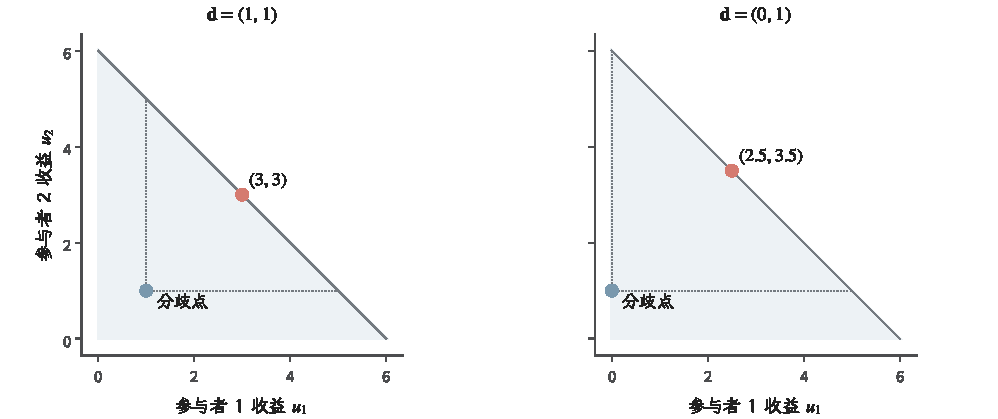
\includegraphics[width=\linewidth]{figures/math-preparation/dynamics/bargaining-disagreement.pdf}
  \caption{两方协商的教学可行域$u_1,u_2\geq0$、$u_1+u_2\leq6$，两图坐标一致。
  蓝点为分歧收益，红点为相对该分歧点的Nash乘积最优解。左图$\bm d=(1,1)$得到
  $(3,3)$，右图$\bm d=(0,1)$得到$(2.5,3.5)$；灰色虚线给出个体可接受的下界。
  可行总收益没有变化，变化的是退出时可得到的收益。}
  \label{fig:game-bargaining-disagreement}
\end{figure*}

没有共同严格正增益时，对数证明不适用，乘积还可能在多个零增益点同时达到最大；若
\(U\)非凸，严格凹性也不能排除不同连通部分上的多个最优点。改变分歧点会改变解，收益
若作一般非线性变换，乘积比较同样会改变。这个“协商解”与非合作博弈中的“Nash均衡”
共享提出者姓名，却解决不同问题。

牌面任务由此可以得到三种互不替代的判断。若参与者对抗，极小极大或Nash均衡检查单方
策略响应；若各方重复学习，遗憾检查相对于某个偏离类的长期损失；若各方合作，Shapley值、
核心或协商解分别按边际贡献、联盟稳定性或分歧点增益分配收益。实际多方系统还可能同时
具有合作与竞争关系，此时必须先写清收益、协调和退出条件，再选择相应解概念。
\section{本章小结}
\label{sec:game-theory-and-multi-agent-decision-summary}
当其他参与者也会选择策略时，行动后果由联合策略决定。有限零和博弈把双方保证值写成
一对线性规划：行方保证收益下界，列方限制收益上界，强对偶使两种证书在同一个博弈值
处相遇。三张牌例子以双方的随机化取得博弈值\(2/3\)，纯策略不能取得这一相互防御。
一般和博弈没有共同博弈值，Nash均衡改为逐人排除单方有利偏离。有限混合策略空间是紧凸
单纯形，Sperner引理与Brouwer定理建立连续不动点，连续近似选择、紧性与闭图再给出
Kakutani路线下的Nash存在性，但不提供唯一性、求解效率或迭代收敛。相关均衡与粗相关
均衡还通过偏离发生在看到建议之前还是之后来区分允许的偏离。
扩展式博弈把行动次序、私人观察和不可区分历史写入信息集。行为策略在每个信息集局部
随机化，Kuhn实现等价说明完全回忆何时使局部表示与完整计划相容。反事实价值去掉自身
到达权重，使少被当前策略访问的信息集仍能比较行动；这种加权不是因果模型中固定外生
背景后的反事实。
重复博弈中的低遗憾是相对于明确比较类的累计保证。投影次梯度由距离平方递推得到
\(O(\sqrt{T})\)外部遗憾；CFR在每个信息集控制即时反事实遗憾。完全回忆使整局偏离
沿本人信息集树分解，由局部正遗憾之和上界全局外部遗憾。两人零和时，加权平均策略趋近
极小极大解；一般和、采样版本和末次迭代需要分别分析。
合作问题改变了待回答的对象。Shapley值在联盟价值已经定义后，平均所有加入次序中的边际
贡献，并由对称性、虚设参与者、有效性和可加性唯一刻画。它不自动保证联盟稳定，
也不把预测归因升级为因果贡献。核心检查联盟是否愿意退出，Pareto条件排除共同改善；
Nash乘积在紧凸且存在共同严格增益时选出唯一收益向量，解仍依赖分歧点。多方决策的结论
须注明收益结构、可用信息、允许偏离和时间口径；只说
“达到均衡”或“分配公平”，不足以确定究竟获得了哪一种保证。
第~\ref{chap:mathematics-and-future-research}章将把前述数学工具按后续研究问题重新组织，
明确不同保证进入学习、推断、迁移与部署时各自控制什么对象。
